%\listfiles
\documentclass[tg]{mdtuffs}
% um tipo específico de monografia pode ser informado como parâmetro opcional:
%\documentclass[tese]{mdtuffs}
% a opção `openright' pode ser usada para forçar inícios de capítulos
% em páginas ímpares
% \documentclass[openright]{mdtuffs}
% para gerar uma versão frente-e-verso, use a opção 'twoside':
% \documentclass[twoside]{mdtuffs}
%\usepackage{hyperref}	
%\usepackage{breakurl}
\usepackage[T1]{fontenc}        % pacote para conj. de caracteres correto
\usepackage{fix-cm}             % para funcionar corretamente o tamanho das fontes da capa
\usepackage{times, color,xcolor}% pacote para usar fonte Adobe Times e cores
\usepackage[utf8]{inputenc}     % pacote para acentuação
\usepackage{graphicx}           % pacote para importar figuras
\usepackage{caption}
\usepackage{subfig}             % para usar várias figuras em subfloats
\usepackage{float}              % para utilizar a opção H nas figuras.
\usepackage[final]{pdfpages}

%\usepackage{pgf,tikz}
%\usepackage{mathrsfs}
%\usetikzlibrary{arrows}
%\pagestyle{empty}

%\usepackage[brazil]{babel}   
\usepackage{enumerate}
\usepackage{amsmath,latexsym,amssymb} %Pacotes matemáticos
\usepackage[%hidelinks%, 
            bookmarksopen=true,linktoc=none,colorlinks=true,
            linkcolor=black,citecolor=black,filecolor=magenta,urlcolor=blue,
            pdftitle={Geração procedural de terrenos com biomas distintos para jogos},
            pdfauthor={João Carlos Becker},
            pdfsubject={Projeto/Trabalho de Conclusão de Curso},
            pdfkeywords={Monografia, Modelo, LaTeX}
            ]{hyperref} %hidelinks disponível no pacote hyperref a partir da versão 2011-02-05  6.82a
%Nesse caso, hidelinks retira os retângulos em volta dos links das referências

%Definição de minha autoria pra funcionar as XML
%\def\lnl#1#2{{\scriptsize\bfseries #1}\hspace{#2em}}
\usepackage{setspace}
%---------------------------------------------------
% Definições dos XML
%---------------------------------------------------
\usepackage{verbatim}
\usepackage{listings}
%\usepackage[usenames,dvipsnames]{color}
	%\def\mlnl#1#2{{\scriptsize\bfseries #1}\hspace{#2em}}

%---------------------------------------------------
% Definições dos Algoritmos
%---------------------------------------------------
	\usepackage[portuguese,ruled,linesnumbered]{algorithm2e}
	\usepackage{etoolbox}
	\makeatletter
	\patchcmd{\@algocf@start}{%
		\begin{lrbox}{\algocf@algobox}%
	}{%
	  \rule{0.\textwidth}{\z@}%
	  \begin{lrbox}{\algocf@algobox}%
	  \begin{minipage}{1.\textwidth}%
	}{}{}
	\patchcmd{\@algocf@finish}{%
	  \end{lrbox}%
	}{%
	  \end{minipage}%-----------------------------------------------------------Tem erro de sintaxe aqui
	  \end{lrbox}%
	}{}{}
	\makeatother

	\SetAlFnt{\tt}
	
	\SetKwFunction{FRecurs}{FnRecursive}%
%-------------------------------------------------

     
\sloppy
%%Margens conforme MDT 1ª edição, arrumar diretamente no mdtuffs.cls para funcionar a opção twoside *PENDENTE*
\usepackage[inner=30mm,outer=20mm,top=30mm,bottom=20mm]{geometry} 

%==============================================================================
% Se o pacote hyperref foi carregado a linha abaixo corrige um bug na hora
% de montar o sumário da lista de figuras e tabelas
% Se o pacote não foi carregado, comentar a linha %
%==============================================================================

%%=============================================================================
%% Trampa para corrigir o bug do hyperref que redefine o caption das figuras e das
%% tabelas, n�o colocando o nome ``Figura'' antes do n�mero do mesmo na lista
%%=============================================================================

\makeatletter

\long\def\@caption#1[#2]#3{%
  \expandafter\ifx\csname if@capstart\expandafter\endcsname
                  \csname iftrue\endcsname
    \global\let\@currentHref\hc@currentHref
  \else
    \hyper@makecurrent{\@captype}%
  \fi
  \@ifundefined{NR@gettitle}{%
    \def\@currentlabelname{#2}%
  }{%
    \NR@gettitle{#2}%
  }%
  \par\addcontentsline{\csname ext@#1\endcsname}{#1}{%
    \protect\numberline{\csname fnum@#1\endcsname ~-- }{\ignorespaces #2}%
  }%
  \begingroup
    \@parboxrestore
    \if@minipage
      \@setminipage
    \fi
    \normalsize
    \expandafter\ifx\csname if@capstart\expandafter\endcsname
                    \csname iftrue\endcsname
      \global\@capstartfalse
      \@makecaption{\csname fnum@#1\endcsname}{\ignorespaces#3}%
    \else
      \@makecaption{\csname fnum@#1\endcsname}{%
        \ignorespaces
        \ifHy@nesting
          \expandafter\hyper@@anchor\expandafter{\@currentHref}{#3}%
        \else
          \Hy@raisedlink{%
            \expandafter\hyper@@anchor\expandafter{%
              \@currentHref
            }{\relax}%
          }%
          #3%
        \fi
      }%
    \fi
    \par
  \endgroup
}

\makeatother

%==============================================================================
% Identificação do trabalho
%==============================================================================
%\title{Geração procedural de biomas}
\title{Geração procedural de terrenos com biomas distintos para jogos}


\author{Becker}{João Carlos}
%Descomentar se for uma "autora"
%\autoratrue

\course{Curso de Ciência da Computação}
\altcourse{Curso de Ciência da Computação}

%não usado por enquanto
\institute{Ciência da Computação}
\degree{Bacharel em Ciência da Computação}

% Número do TG (verificar na secretaria do curso)
% Para mestrado deixar sem opção dentro do {}
\trabalhoNumero{}

%Orientador
\advisor[Prof.]{Dr.}{Wuerges}{Emílio}
%Se for uma ``orientadora'' descomentar a linha baixo
%\orientadoratrue

%Co orientador, comentar se não existir
%\coadvisor[Prof.]{Drª.}{Pereira}{Maria Regina}
%\coorientadoratrue %Se for uma ``Co-Orientadora''

%Avaliadores (Banca)
\committee[Dr.]{de Mello}{Braulio Adriano}{UFFS}
\committee[Dr.]{Bins Filho}{José Carlos}{UFFS}

% a data deve ser a da defesa; se nao especificada, são gerados
% mes e ano correntes
\date{11}{Dezembro}{2017}

%Palavras chave
%\keyword{Dissertação} 
%\keyword{Modelo}
%\keyword{LaTeX}

%%=============================================================================
%% Início do documento
%%=============================================================================
\begin{document}

%%=============================================================================
%% Capa e folha de rosto
%%=============================================================================
\maketitle

%%=============================================================================
%% Catalogação e Folha de aprovação DEBUG: descomentar isso
%%=============================================================================
\clearpage
%Somente para TCC 2: Está página deve ser substituida pela ficha de catalogação antes de sua entrega na biblioteca. 
%Somente obrigatório para dissertação, para TG, remover as linhas	77	%
%Como a CIP vai ser impressa atrás da página de rosto, as margens inner e outer	
%devem ser invertidas.
\newgeometry{inner=20mm,outer=30mm,top=30mm,bottom=20mm}	
\makeCIP{joaoc.becker@hotmail.com} %email do autor		
\restoregeometry

%Se for usar a catalogação gerada pelo gerador do site da biblioteca comentar as linhas
%acima e utilizar o comando abaixo
%\includeCIP{CIP.pdf}

%folha de aprovação

%IMPORTANTE: Esta folha deverá ser impressa e assinada pela banca e depois digitalizada e inserida no arquivo final para entrega no repositório institucional.
%\makeapprove
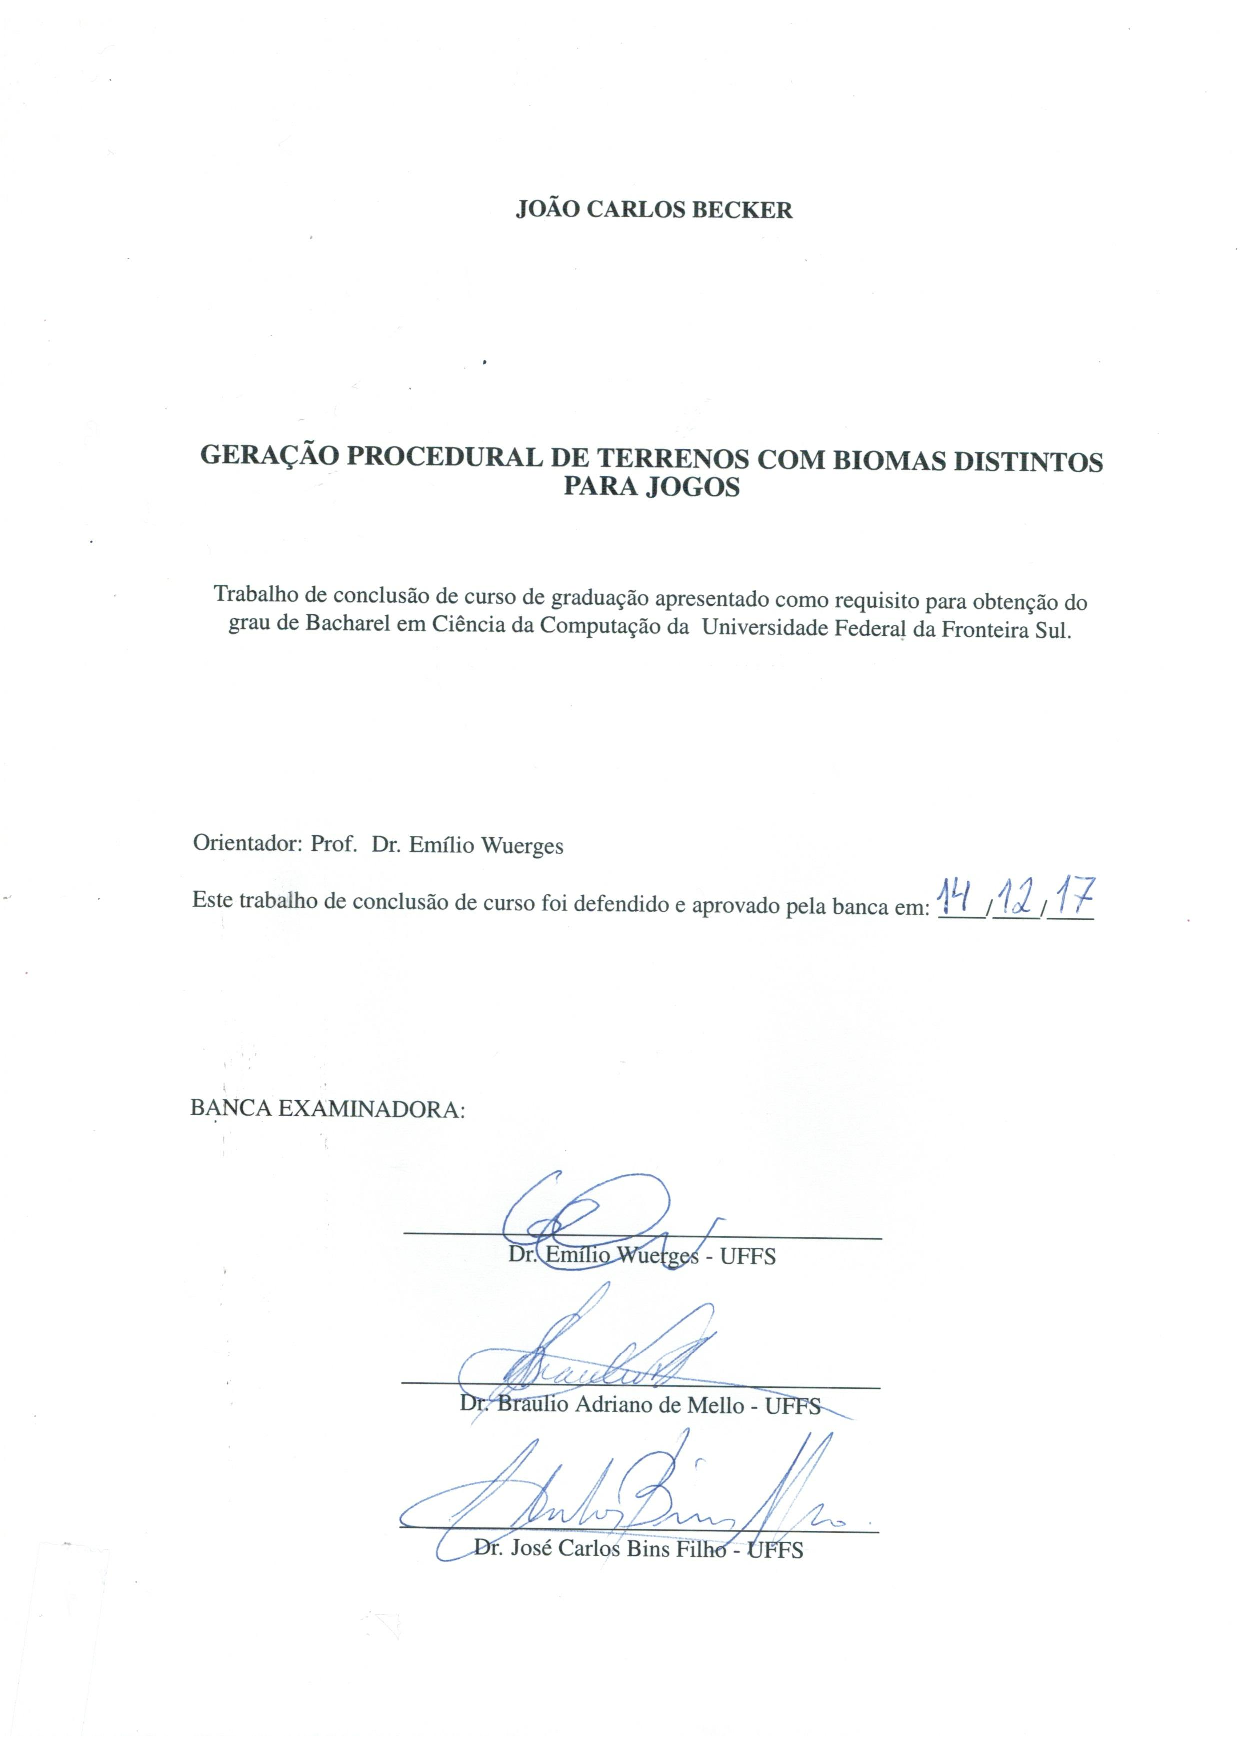
\includepdf[]{scan.pdf}

%%=============================================================================
%% Dedicatória (opcional)
%%=============================================================================
%\clearpage
%\begin{flushright}
%\begin{onehalfspacing}
%\mbox{}\vfill

%{Texto da dedicatória ......}

%\end{onehalfspacing}
%\end{flushright}

%%=============================================================================
%% Agradecimentos (opcional)
%%=============================================================================
%\clearpage
%{
%\centering
%\textbf{AGRADECIMENTOS}\\
%}
%\vspace{1.5cm}
%\begin{onehalfspacing}

%Texto de agradecimento. 

%\end{onehalfspacing}


%%=============================================================================
%% Epígrafe (opcional)
%%=============================================================================
%\clearpage
%\begin{flushright}
%\mbox{}\vfill
%{\sffamily\itshape
%``Frase da epígrafe'' \\ }
%--- \textsc{Autor da frase}
%\end{flushright}


%%=============================================================================
%% Resumo
%%=============================================================================
\begin{abstract}
    Quanto maior o cenário de um jogo, mais tempo o jogador irá explorá-lo.
    Tradicionalmente, esta demanda é suprida através de uma grande equipe de design gráfico.
    Neste trabalho é apresentada uma técnica capaz de gerar proceduralmente um terreno pseudo-infinito
    com 5 biomas visualmente distintos, distribuí-los em regiões e suavizar suas fronteiras.
    A área, a frequência, a adjacência, a suavidade dos biomas pode ser ajustada
    através de parâmetros.
    O resultado é um gerador de terrenos adequado para uso no desenvolvimento de jogos de computador.
    \keyword{Geração procedural de conteúdo}
    \keyword{Mapas de altura}
    \keyword{jogos 3D}
\end{abstract}










%%=============================================================================
%% Abstract
%%=============================================================================
% resumo na outra língua
% como parametros devem ser passados o titulo, o nome do curso,
% as palavras-chave na outra língua, separadas por vírgulas, o mês em inglês
%o a sigla do dia em inglês: st, nd, th ...
\begin{englishabstract}
{Biome procedural generation}
{Bachelor of Computer Science}
{Procedural Content Generation, Height maps, 3D games}
{July}
{fr}
    The larger the scenario of a game, more time a player will spend to exploit it.
    Traditionally,  computer games scenarios were built using large graphic design teams.
    This work details a technique able to procedurally generate a pseudo-infinite terrain, with 5 visually distinct biomes,
    spread them in regions and smooth their borders.
    The area, frequency, adjacency and smoothness of the biomes and the terrain can be adjusted through parameters.
    The resulting work is a terrain generator suited for computer games development.
\end{englishabstract}

%% Lista de Ilustrações (opc)
%% Lista de Símbolos (opc)
%% Lista de Anexos e Apêndices (opc)

%%=============================================================================
%% Lista de figuras (comentar se não houver)
%%=============================================================================
\listoffigures

%%=============================================================================
%% Lista de tabelas (comentar se não houver)
%%=============================================================================
\listoftables

%%=============================================================================
%% Lista de Apêndices (comentar se não houver)
%%=============================================================================
%\listofappendix

%%=============================================================================
%% Lista de Anexos (comentar se não houver)
%%=============================================================================
%\listofannex

%%=============================================================================
%% Lista de abreviaturas e siglas
%%=============================================================================
% O parametro deve ser a abreviatura mais longa
\begin{listofabbrv}{OpenGL}
    \item [GDP] Produto Interno Bruto \textit{(Gross Domestic Product)}
    \item [OpenGL] \textit{Open Graphics Library}
    \item [GLSL] \textit{OpenGL Shading Language}
    \item [ESA] \textit{Entertainment Software Association}
    \item [GDP] \textit{Gross domestic product}
    \item [PCG] \textit{Procedural Content Generation}
    \item [fps] Quadros por segundo
    
%   \item [BNF] \textit{Backus-Naur Form}
%  \item [UbiComp] Computação Ubíqua
\end{listofabbrv}


%%=============================================================================
%% Lista de simbolos (opcional)
%%=============================================================================
%Simbolos devem aparecer conforme a ordem em que aparecem no texto
% o parametro deve ser o símbolo mais longo
\begin{listofsymbols}{$\Delta_{v}$}
    \item [$V$] vetor de vértices
    \item [$E$] vetor de índices em $V$
    \item [$\Delta_{v}$] Distância entre vérticies adjacentes projetados no plano $X \times Z$
    \item [$k$] Quantidade de vértices será $k^2$
    \item [$x_{s}$] Ponto inicial no eixo $X$ para determinada \textit{chunk}
    \item [$z_{s}$] Ponto inicial no eixo $Z$ para determinada \textit{chunk}
    \item [$b$] Tamanho de bioma
    \item [$l$] Distância de fronteira
    \item [$h'$] Retorno de ruído
    \item [$\theta$] Quantidade de \textit{octaves}
    \item [$f$] Frequência de ruído
    
\end{listofsymbols}

%%=============================================================================
%% Sumário
%%=============================================================================
\tableofcontents


%%=============================================================================
%% Início da monografia
%%=============================================================================
\setlength{\baselineskip}{1.5\baselineskip}

%Adiciona cada capitulo
\begin{frame}{Problemática}
    \begin{itemize} \setlength\itemsep{1em}
        \item Os jogos digitais estão cada vez melhores e exigindo mais
        complexidade para os mesmos, trazendo mais conteúdo agregado.
        \item O tempo para produzir este conteúdo demanda muito esforço de trabalho.
    \end{itemize}
\end{frame}


%\begin{frame}{Introdução}
%    
%\end{frame}

\begin{frame}{Objetivos}
    \begin{itemize}
        \item Objetivo Geral
        \begin{itemize}
            \item Este projeto tem como objetivo gerar mapas de tamanho pseudo-infinitos, com 
            relevo gerado proceduralmente usando ruído 
            de Perlin, de maneira não assistida, os mapas de altura devem representar o 
            relevo de pelo menos dois biomas arbitrários com fronteiras contínuas.
        \end{itemize}
        \item Objetivos Específicos
        \begin{itemize}
            \item Implementar malhas da superfície com tamanho pseudo-infinito;
            \item Selecionar biomas, e as características dos mesmos a ser representadas;
            \item Construir algoritmo para manipular ruído de Perlin e gerar características
                selecionadas do bioma;
            \item Gerar divisões entre biomas sobre a malha de regiões;
            \item Implementar fronteiras contínuas entre biomas;
            \item Comparar resultado com cenários de jogos.
        \end{itemize}
    \end{itemize}
\end{frame}
\chapter{Referencial Teórico}
Neste Capítulo, serão abordados alguns conceitos e técnicas necessárias para
compreender o trabalho proposto, que é 
gerar malha e mapa de altura com tamanho pseudo-infinitos, de maneira procedural
e não assistida, suportando mais de um bioma.

\section{Biomas}
Neste trabalho o conceito de bioma vai ser outro, o resultado deste
vai ser unicamente mapas de altura, então a única característica que é relevante
são as altitudes do solo e seus padrões, descartando dados como tipo da
vegetação e sua distribuição, umidade e entre outros. Então no restante 
do trabalho, quando for usado os termos "característica do bioma", o mesmo vai
se referir a alguma característica de altitude do bioma. A cor será um segundo auxílio
para ajudar na percepção de biomas distintos em um mapa.

Para fins de restringir o escopo do projeto vamos agrupar os biomas por padrões
de relevo e não por fauna e flora como feito nos conceitos mais conhecidos.

Como este trabalho é voltado para a área de jogos, dentro da comunidade de jogadores
é bem aceito usar o termo bioma de forma mais genérica. O jogo Minecraft usa o
termo e entre seus biomas se encontra \textit{Extreme Hills} e \textit{Plains}.

Normalmente jogos tem um padrão de arte, os biomas que neles são mostrados não 
precisam ser realistas e nem respeitar a natureza real ou as regras da física. Aqui será 
abordado a implementação de uma técnica que consiste separar regiões de biomas, e criar
um terreno aplicável para jogos com múltiplos biomas.

\section{Representação das Regiões}
%Um bioma vai pertencer a um conjunto de regiões, na imagem \ref{fig:squadStripBiomes}
%que usa uma malha de quadrados, onde os segmentos de retas vermelhas são fronteiras entre
%biomas.
A maneira de separar regiões de biomas será com áreas quadradas, cada uma delas com
tamanho $b^{2}$, cada região tem um identificador $(dxs, dzs)$, esse identificador
será usado como entrada em uma função de ruído, O valor deste retornado deste ruído vai 
determinar o bioma da região em questão. Na figura \ref{fig:squadStripBiomes} temos
um exemplo com várias regiões, algumas dessas regiões fazendo fronteira entre biomas, 
nela é visível 3 biomas distintos.

\begin{figure}[H]
    \centering
    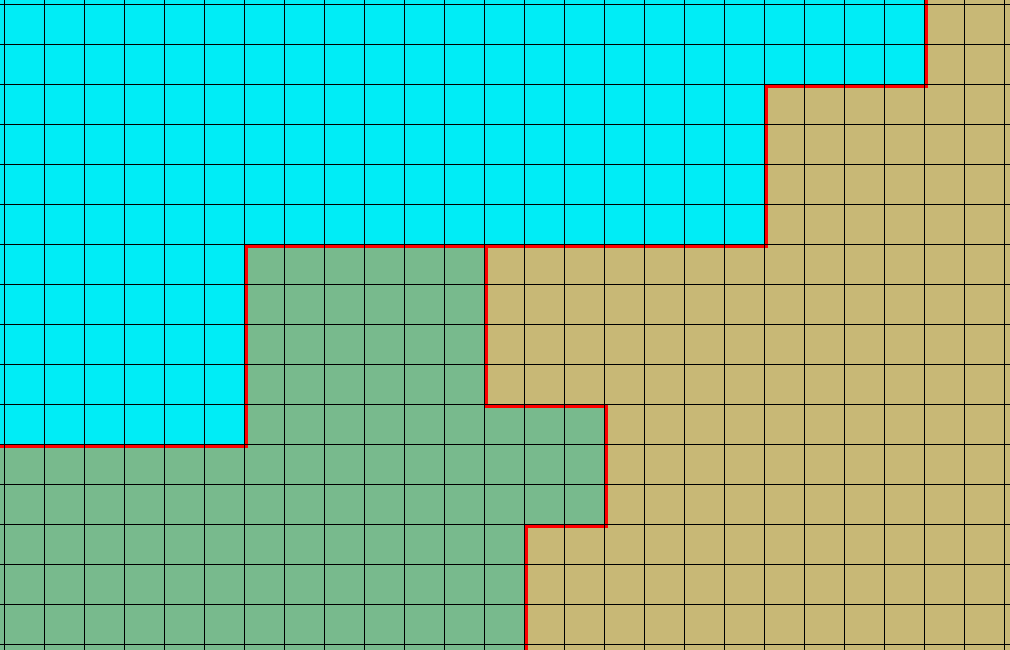
\includegraphics[width=0.7\textwidth]{figuras/squadStripBiomes.png}
    \caption{Malha de quadrados com divisão de biomas}
    \label{fig:squadStripBiomes}
\end{figure}
\section{Malha de terrenos}
\subsection{Malhas de quadrado}
Este modelo é apresentado na figura \ref{fig:squadStripBiomes}, nele cada
quadrado é uma região. Os vértices armazenados se encontram nos quatro cantos
do quadrado, então um vértice é comum a quatro quadrados, cada um deles
compartilhando o vértice com os quadrados adjacentes, as arestas entre vértices
vizinhos são uma fronteira entre regiões, e tem a possibilidade desta aresta ser
também uma fronteira entre biomas.

Devido ao padrão podemos perceber que não há necessidade de armazenar arestas
em memória, já que a mesma só vai existir entre vértices vizinhos, o vértice
$v_{i, j}$ tem como vizinhos o conjunto $\{v_{i+1, j}, v_{i-1, j}, v_{i, j+1}, v_{i, j-1}\}$.
\subsection{Malha triangular}
Usando a mesma base de vértice da malha de quadrados, agora temos uma aresta
adicional, uma diagonal em cada quadrado do modelo anterior, dividindo a região
em duas, cada triangulo sendo uma região, como podemos ver na figura \ref{fig:vbo}.
Agora além do conjunto de arestas do modelo anterior, o vértice $v_{i, j}$ também tem
aresta para os vértices $\{v_{i+1, j+1}, v_{i-1, j-1}\}$.

\begin{figure}[H]
    \centering
    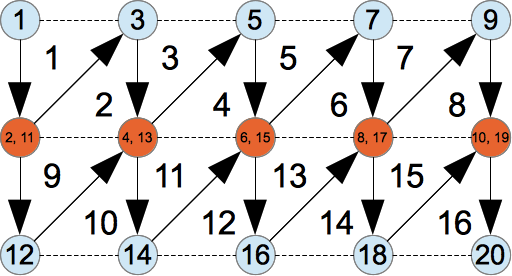
\includegraphics[width=0.5\textwidth]{figuras/vbo.png}
    \caption{Malhas de triângulos, retirado de \cite{androidtrianglestrip}}
    \label{fig:vbo}
\end{figure}

O terreno precisa ser formado por polígonos, para que seja possível renderizar pedaços de planos.
Se a quantidade de vértices por polígono for maior que $3$, então tem pelo menos um ponto com altura sendo uma 
variável não livre.
%\subsection{Diagrama de Voronoi}
%Um diagrama de Voronoi é uma partição no plano para separar regiões, recebendo
%como entrada um conjunto de pontos chamados de \textit{sites}, o algoritmo
%separa as regiões de cada \textit{site} deixando a fronteira equidistante entre eles
%\cite{fortune1987sweepline}.
%
%Como está implementação vai ser não assistida estes sites precisam ser colocados
%aleatoriamente e proceduralmente, para não ocorrer aglomerações de site, já
%que existe a possibilidade de acontecer na geração de \textit{sites} aleatórios,
%será usado o algoritmo de Lloyd's para relaxar os sites, o conjunto dessas
%técnicas já foi usado por \cite{patel2010polygonal}, para gerar malha de regiões,
%segue uma imagem de seu diagrama na figura \ref{fig:voronoi-2-lloyd}, este diagrama
%foi usado para alcançar o resultado já mostrado na ilustração \ref{fig:voronoi-map-goal-distorted}.
%\begin{figure}[H]
%    \centering
%    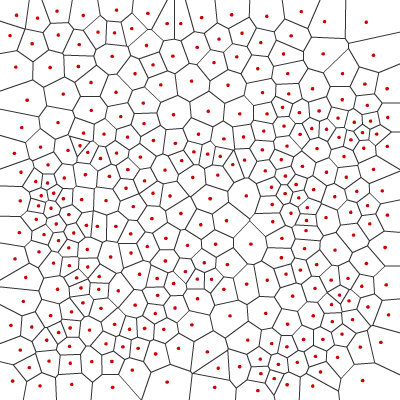
\includegraphics[width=0.5\textwidth]{figuras/voronoi-2-lloyd.png}
%    \caption{Diagrama de Voronoi com algoritmo de Lloyd's aplicado, por \cite{patel2010polygonal}}
%    \label{fig:voronoi-2-lloyd}
%\end{figure}

\section{Ruído de Perlin}
Bons geradores de números aleatórios geram números onde não existe relação entre
eles, porem se montado um gráfico com eles, o resultado não teria um aspecto
orgânico, então para o terreno ter um relevo mais parecido com o encontrado na 
natureza é usado uma função de ruído \cite{shiffman2012nature}, está comparação
pode ser feita com a imagem \ref{fig:randomAndNoise}. 
\begin{figure}[H]
    \centering
    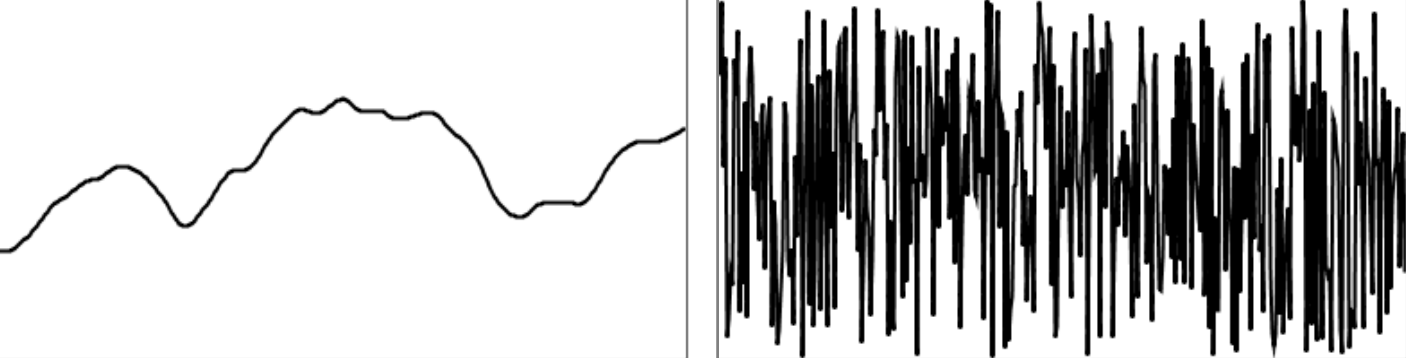
\includegraphics[width=0.7\textwidth]{figuras/randomAndNoise.png}
    \caption{Da esquerda, função de ruído, função de pontos aleatórios. Por \cite{shiffman2012nature}}
    \label{fig:randomAndNoise}
\end{figure}

Uma função de ruído recebe como parâmetro as coordenadas em um espaço de $n$ dimensões e
retorna um valor entre $-1$ e $1$ para tal posição\cite{shiffman2012nature}.

Na figura \ref{fig:randomAndNoise} vimos o ruído unidimensional, o ruído
tem a complexidade $O(2^n)$, sendo $n$ a quantidade de dimensões \cite{zucker2001perlin}.
Este mesmo ruído unidimensional pode ser usado nas fronteiras entre biomas, dando
um aspecto mais natural á fronteiras, da mesma maneira que foi usado nas bordas
das ilhas no trabalho de \cite{patel2010polygonal}. Contudo, para gerar altura
em um cenário tridimensional precisamos usar o ruído bidimensional. Existem
implementações do ruído em placas gráficas que calculam a função de ruído para 
$\{1, 2, 3\}$ dimensões em único ciclo \cite{perlin2002improving}.

No ruído unidimensional a resposta é uma interpolação entre os seus vizinhos, que
neste caso são apenas $2$. Caso o parâmetro do ruído for $x_{i}$, o mesmo só tem 
como vizinhos, $x_{i+1}$ e $x_{i-1}$, quando a dimensão aumenta e por conta disso
os parâmetros também, a quantidade de vizinhos também aumenta \cite{shiffman2012nature}, 
como o mesmo exemplifica na ilustração \ref{fig:1dto2dnoise}.
\begin{figure}[H]
    \centering
    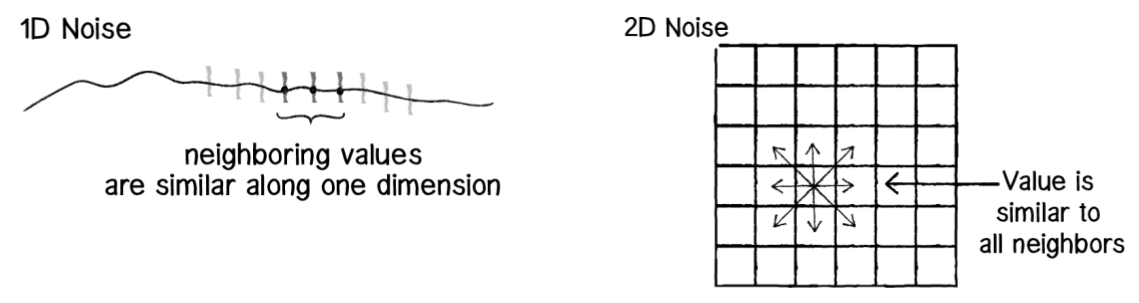
\includegraphics[width=0.7\textwidth]{figuras/1dto2dnoise.png}
    \caption{Vizinhas para função de ruído, $1d$ para $2d$. Por \cite{shiffman2012nature}}
    \label{fig:1dto2dnoise}
\end{figure}

O \textit{ruído de Perlin} usa a função ruído várias vezes, cada uma é chamada
de oitava. Oitava usa amplitude e frequência diferente, a quantidade de oitavas
usada varia de implementações para necessidades, a primeira oitava é gerada com uma
amplitude alta e frequência baixa, as próxima oitava tem a metade da amplitude e 
o dobro da frequência, o ruído de Perlin é a soma de todas as oitavas computadas,
adaptado de Hugo Elias \cite{carli2012canion} gerou as imagens
\ref{fig:perlin1d} e \ref{fig:perlin2d} do ruído de Perlin em uma e duas
dimensões respectivamente.
\begin{figure}[H]
    \centering
    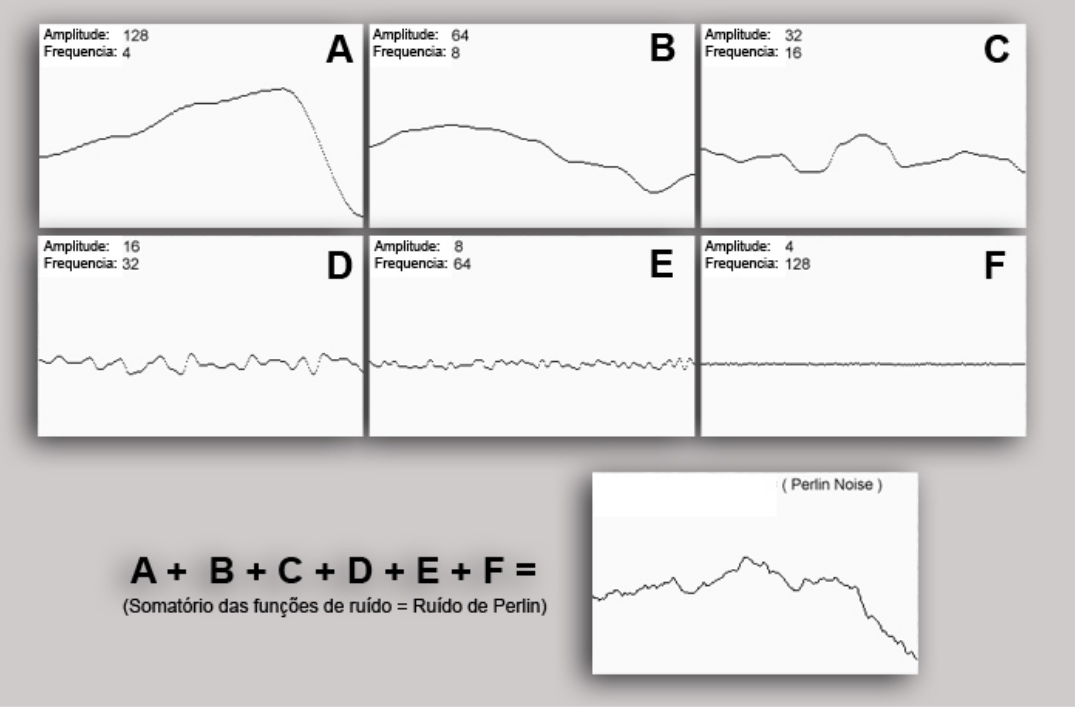
\includegraphics[width=0.7\textwidth]{figuras/perlin1d.png}
    \caption{Gerando ruído de Perlin para uma dimensão}
    \label{fig:perlin1d}
\end{figure}
\begin{figure}[H]
    \centering
    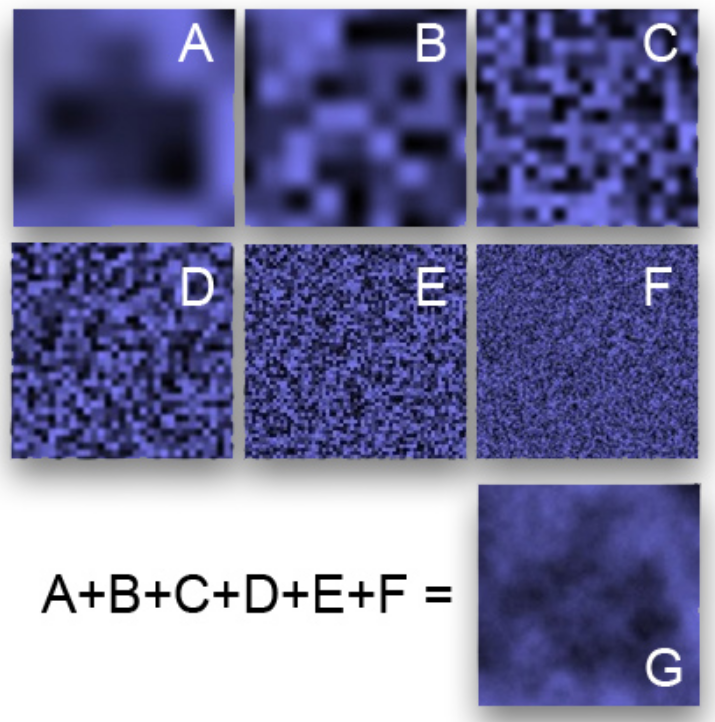
\includegraphics[width=0.6\textwidth]{figuras/perlin2d.png}
    \caption{Gerando ruído de Perlin para duas dimensões}
    \label{fig:perlin2d}
\end{figure}

\section{Mapas de Altura}
Mapas de altura é uma maneira de representar altitudes de um terreno, e essa
será uma das saídas desta implementação proposta, mapas de altura costumam ser, imagens
onde os pontos mais claros representam pontos mais elevados e os escuros regiões mais baixas.
A imagem \ref{fig:perlin2d} já traz exemplos de mapas de altura.

Um mapa de altura pode ser usado para ser renderizado em diferentes perspectivas,
ou para usar processos que geram imagens de luz e sombra, ilustrados na figura \ref{fig:hmap} de \cite{dachsbacher2006interactive}.
\begin{figure}[H]
    \centering
    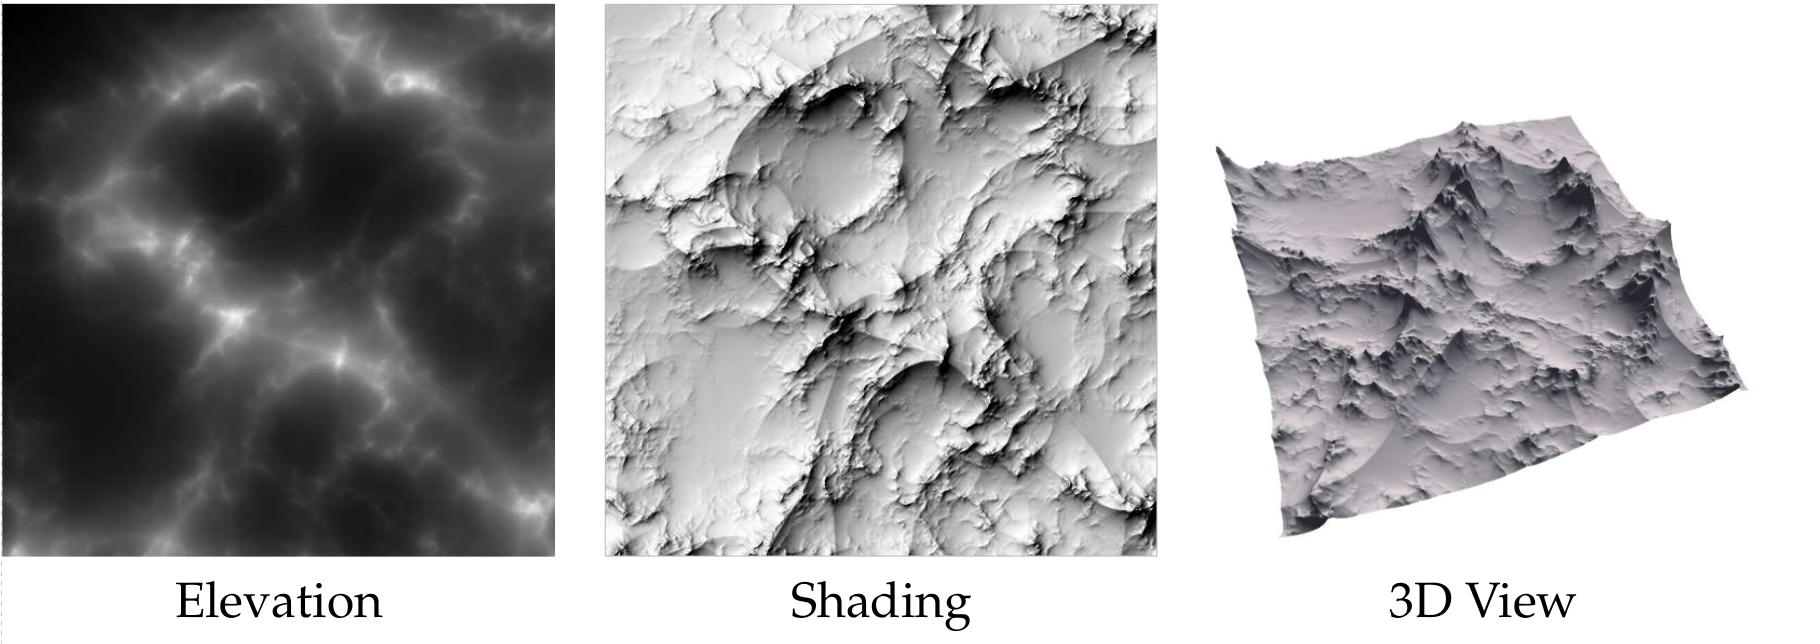
\includegraphics[width=0.75\textwidth]{figuras/hmap.png}
    \caption{Diferentes maneiras de usar um mapa de altura por \cite{dachsbacher2006interactive}}
    \label{fig:hmap}
\end{figure}

%trabalhos correlatos
%gerador de costas do fenando
%voronoi do indiano
\section{Trabalho de Carli}
O trabalho do \cite{carli2012canion} não só gera o mapa de altura, mas também
faz busca de percursos de rio e agentes no mapa. As maiores semelhanças deste 
trabalho com o proposto, é que se faz uso da manipulação dos resultados do ruído de
de Perlin para recriar alguns padrões de relevo e também é uma técnica não assistida.
Entretanto no projeto que 
estou propondo se faz necessário ter pelo menos duas manipulações de ruído distintas
e criar fronteiras contínuas quando as mesmas se encontram, o trabalho 
do \cite{carli2012canion} se preocupa com os parâmetros usados no ruído e manipulação do
resultado, já que o objetivo dele foi criar cânyons realistas, aqui estes parâmetros serão arbitrários
sem a intensão de criar terrenos realistas, mas sim propor uma técnica que cria terreno de múltiplos biomas com fronteira suaves.


%\chapter{Metodologia}
Nesta seção veremos a metodologia do trabalho desde a busca por fontes e trabalhos
relacionados até a analise de resultados.

Começando pela leitura de trabalhos relacionados, os primeiros trabalhos lidos
foram recomendados por professores, a partir destes trabalhos li algumas de suas
referências mais relevantes, os mesmos continham outras citações relevantes, e
assim por diante, dessa maneira, tenho em mãos uma "árvore" de citações,
para preencher algumas lacunas e reforçar alguns argumentos foram necessárias
mais buscas de artigos e trabalhos.

%Selecionar maneira de separar regiões;
A primeira etapa da implementação é escolher a maneira em que regiões serão
separadas, um bioma vai pertencer a um conjunto de regiões, as opções
pré-selecionadas são: \textit{Triangle strip}, malha de quadrados e diagrama de
voronoi. Cada uma delas tem sua vantagem, diagrama de voronoi constrói fronteiras
mais naturais, as outras técnicas tem implementação mais fácil, menor custo
computacional e geram a possibilidade de trabalhar com mapas pseudo infinitos.
Então serão implementadas as três e feitas comparações sobre elas para decidir
qual a melhor opção. A decisão será tomada...
NÃO FAÇO A MENOR IDEIA DE COMO ESSA DECISÃO VAI SER FEITA.

%Selecionar biomas, e as características dos mesmos a ser representadas;
Próxima etapa é a escolha de biomas e suas características a serem geradas pelo%estou repetindo de mais a palavra caracteristica, preciso dar um jeito nisso
algoritmo, a principio a escolha será feita por características fáceis de
implementar, biomas com características mais distintas, para ser visualmente
mais fácil de distinguir regiões de um e outro.%Construir algoritmo para manipular ruído de Perlin e gerar características selecionadas do bioma;
E como já visto no trabalho de \cite{carli2012canion}, podemos manipular o ruído
de Perlin para imitar as características de alguns padrões da natureza, então, 
o mesmo será feito para os biomas selecionados.

%Implementar fronteiras contínuas entre biomas;
Caso não tratado, as fronteiras em biomas podem e provavelmente serão
descontinuas, tendo uma mudança brusca de altura nas fronteiras e deixando o
cenário sem sentido, então nesta etapa será analisadas as possibilidades para
correção da descontinuidade e implementar a mesma.

%Comparar resultado com cenários de jogos e Comparar resultados com a natureza.
\chapter{Resultados}

\begin{figure}[H]
    \centering
    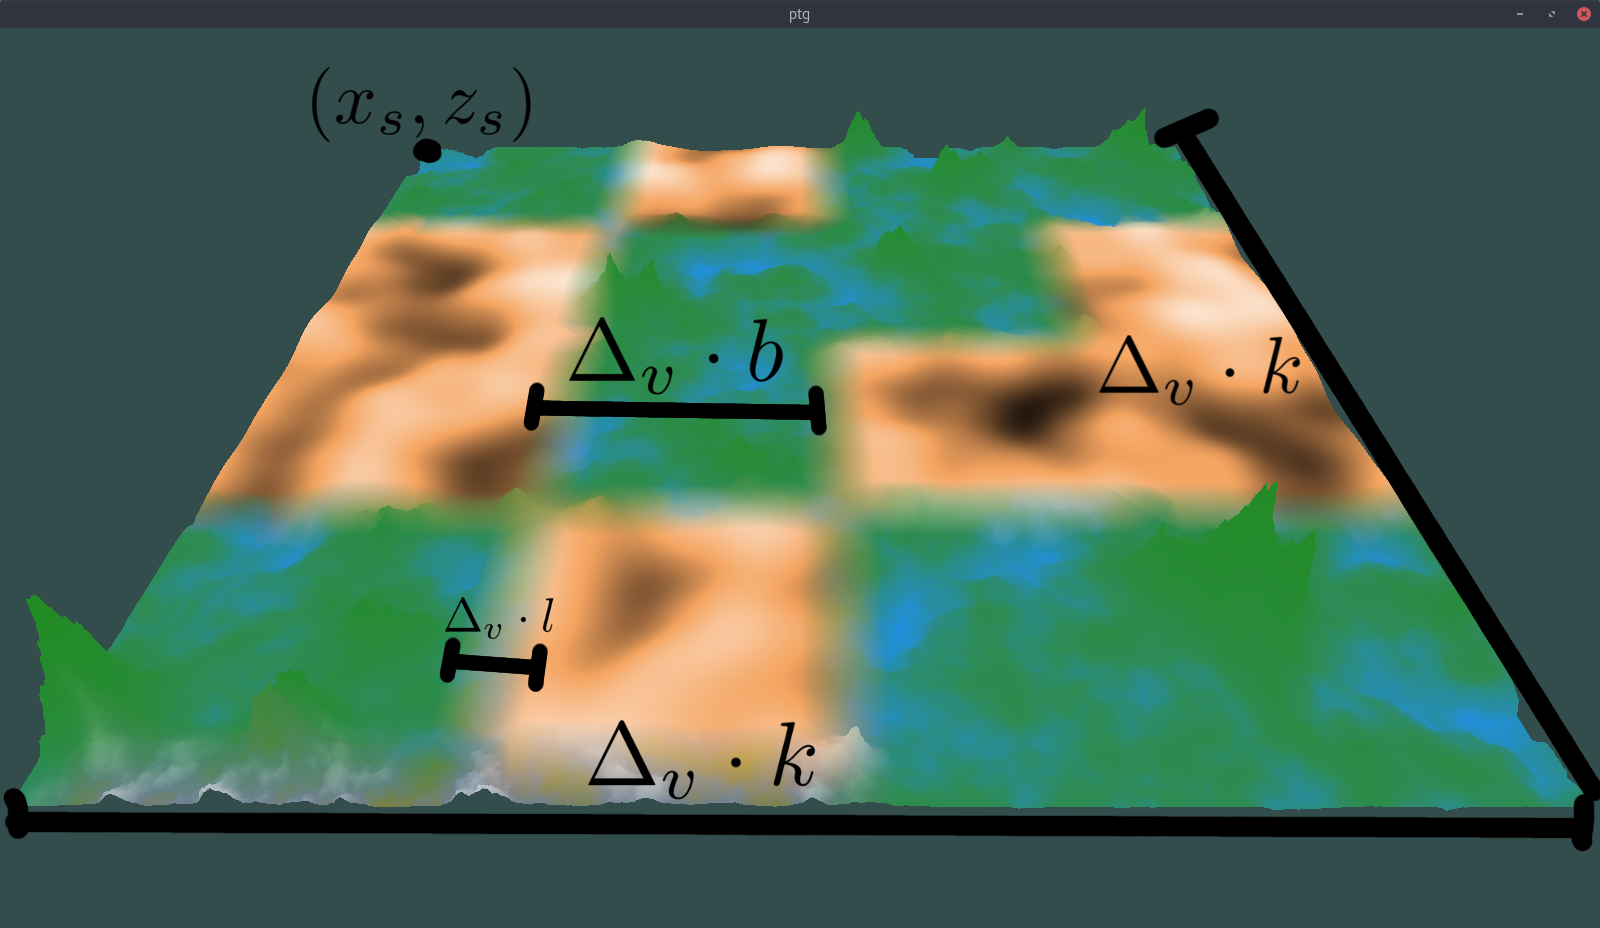
\includegraphics[width=0.75\textwidth]{figuras/resultados/sseditada.png}
    \caption{sseditada}
    \label{fig:sseditada}
\end{figure}


\begin{figure}[H]
    \centering
    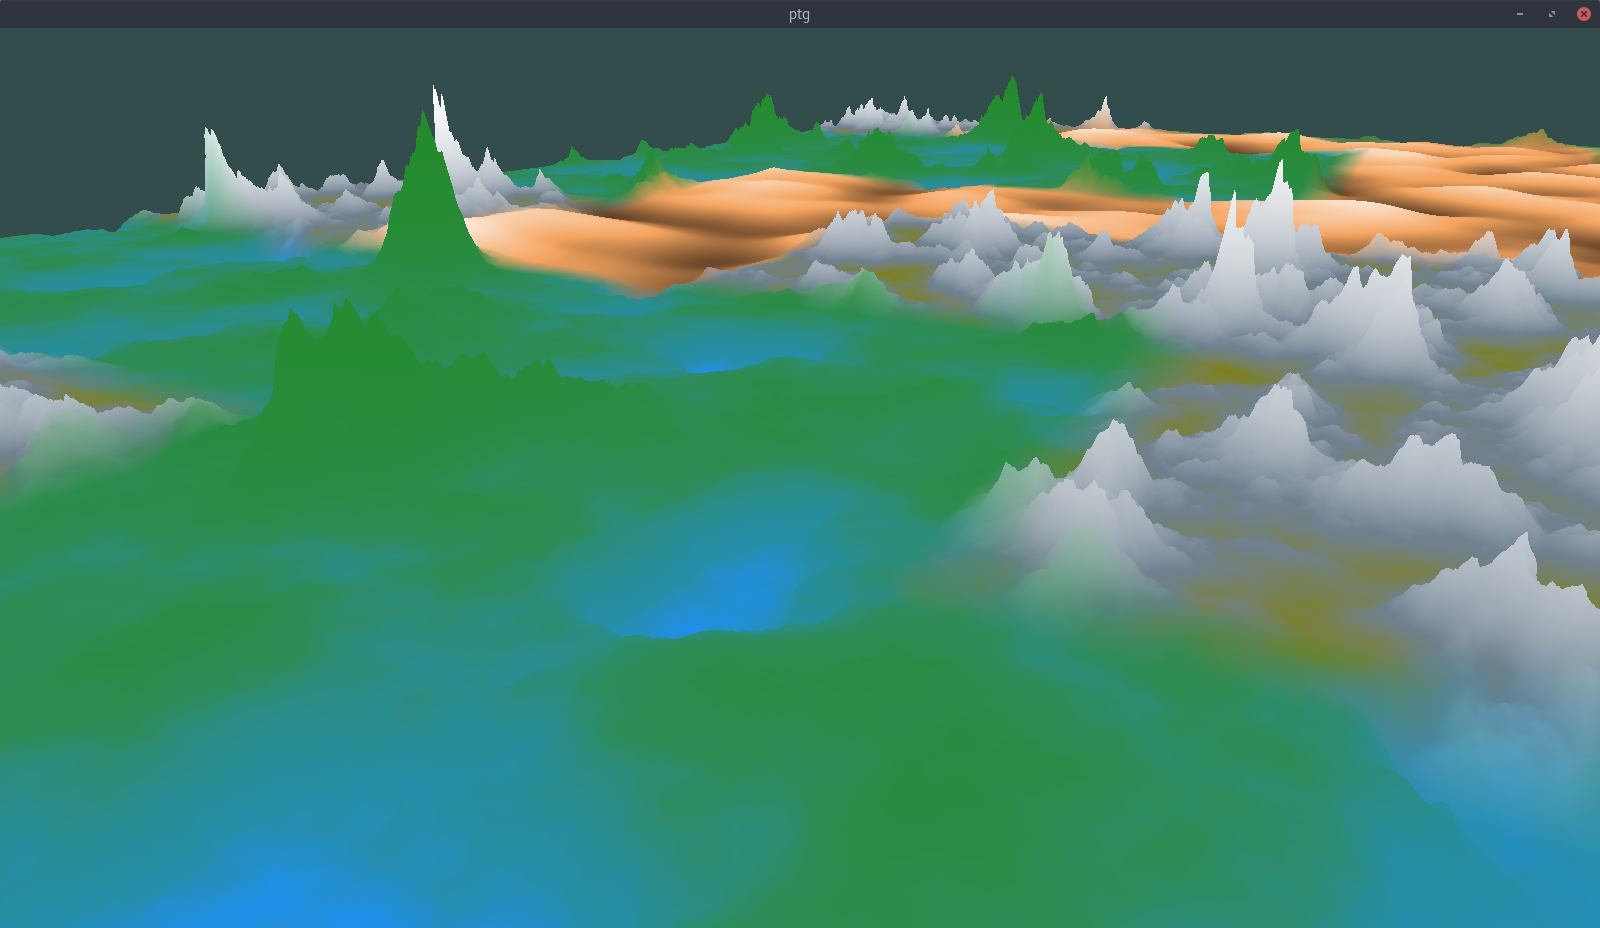
\includegraphics[width=0.5\textwidth]{figuras/ssFinalResult.png}
    \caption{Resultado final}
    \label{fig:ssFinalResult}
\end{figure}

\begin{figure}[H]
     \centering
     \subfloat[][$b = 260$]{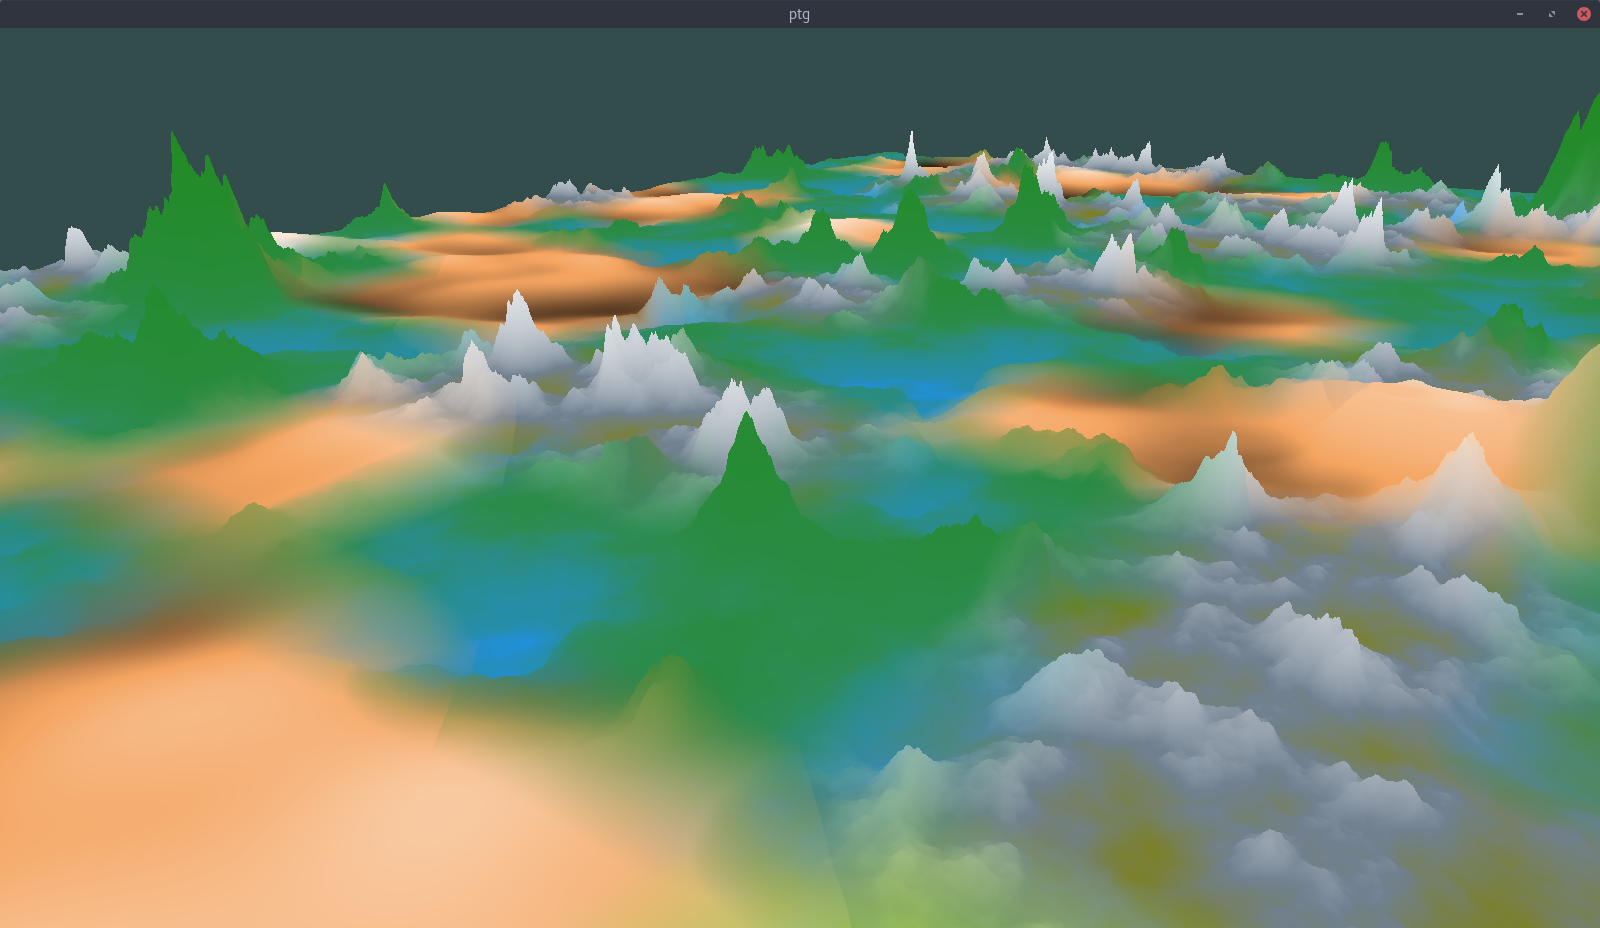
\includegraphics[width=0.48\textwidth]{figuras/resultados/b/resultSeed3Deltav05k2048b260l128.png}\label{fig:b260}}\hspace{0.1cm}
     \subfloat[][$b = 512$]{\includegraphics[width=0.48\textwidth]{figuras/resultados/b/resultSeed3Deltav05k2048b512l128.png}\label{fig:b512}}\\
     \subfloat[][$b = 1024$]{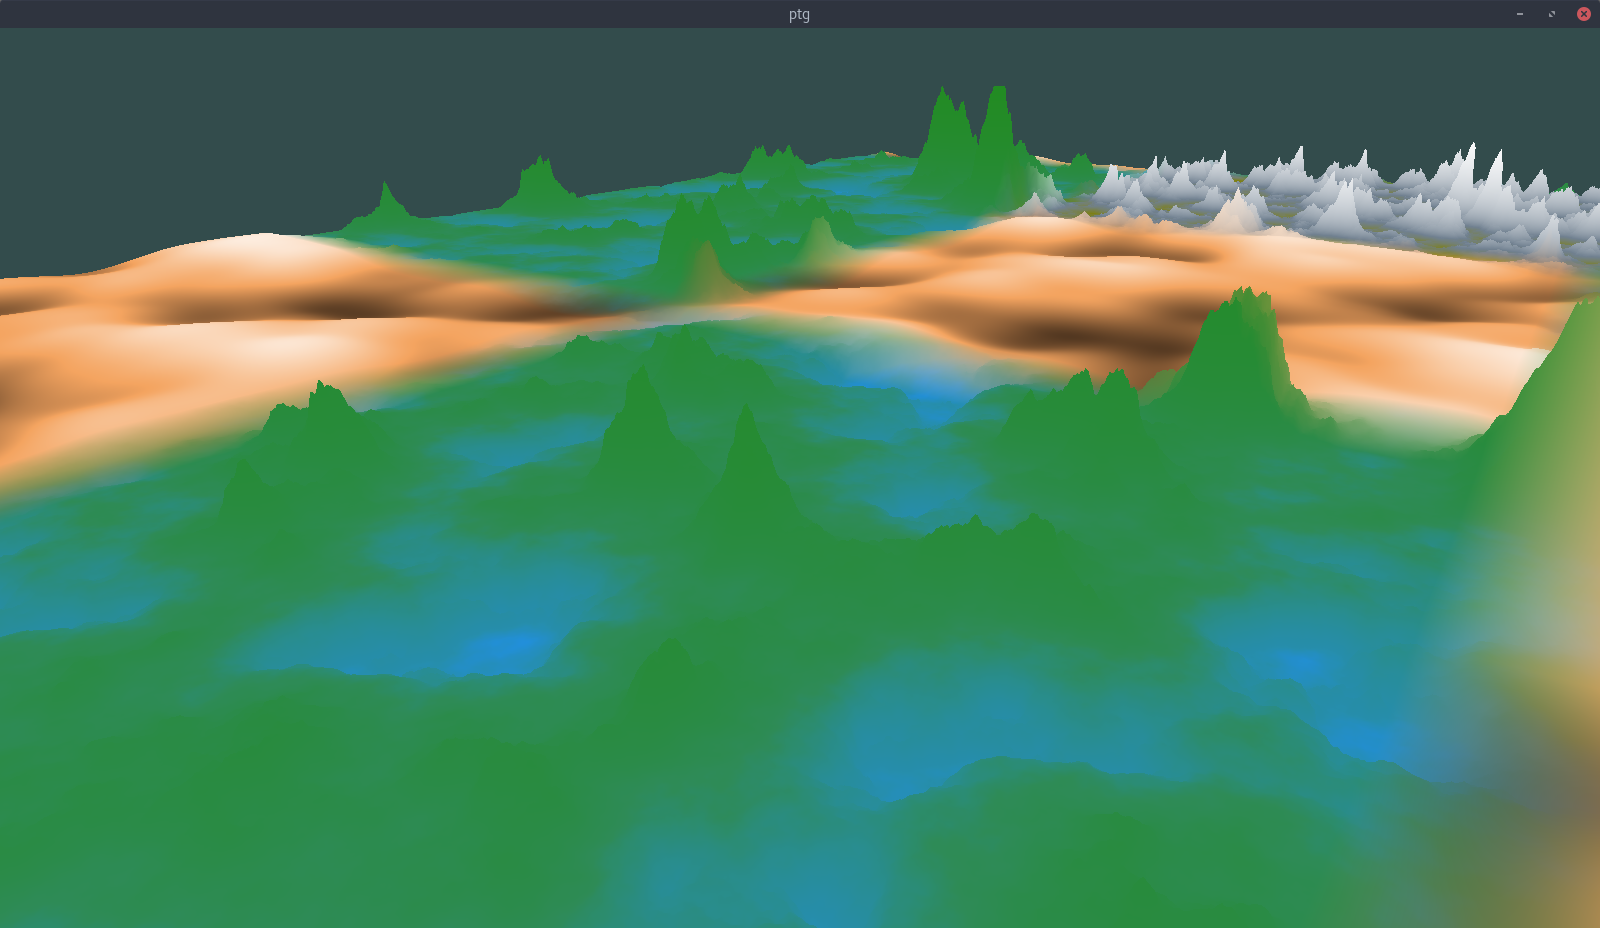
\includegraphics[width=0.48\textwidth]{figuras/resultados/b/resultSeed3Deltav05k2048b1024l128.png}\label{fig:b1024}}\hspace{0.1cm}
     \subfloat[][$b = 1500$]{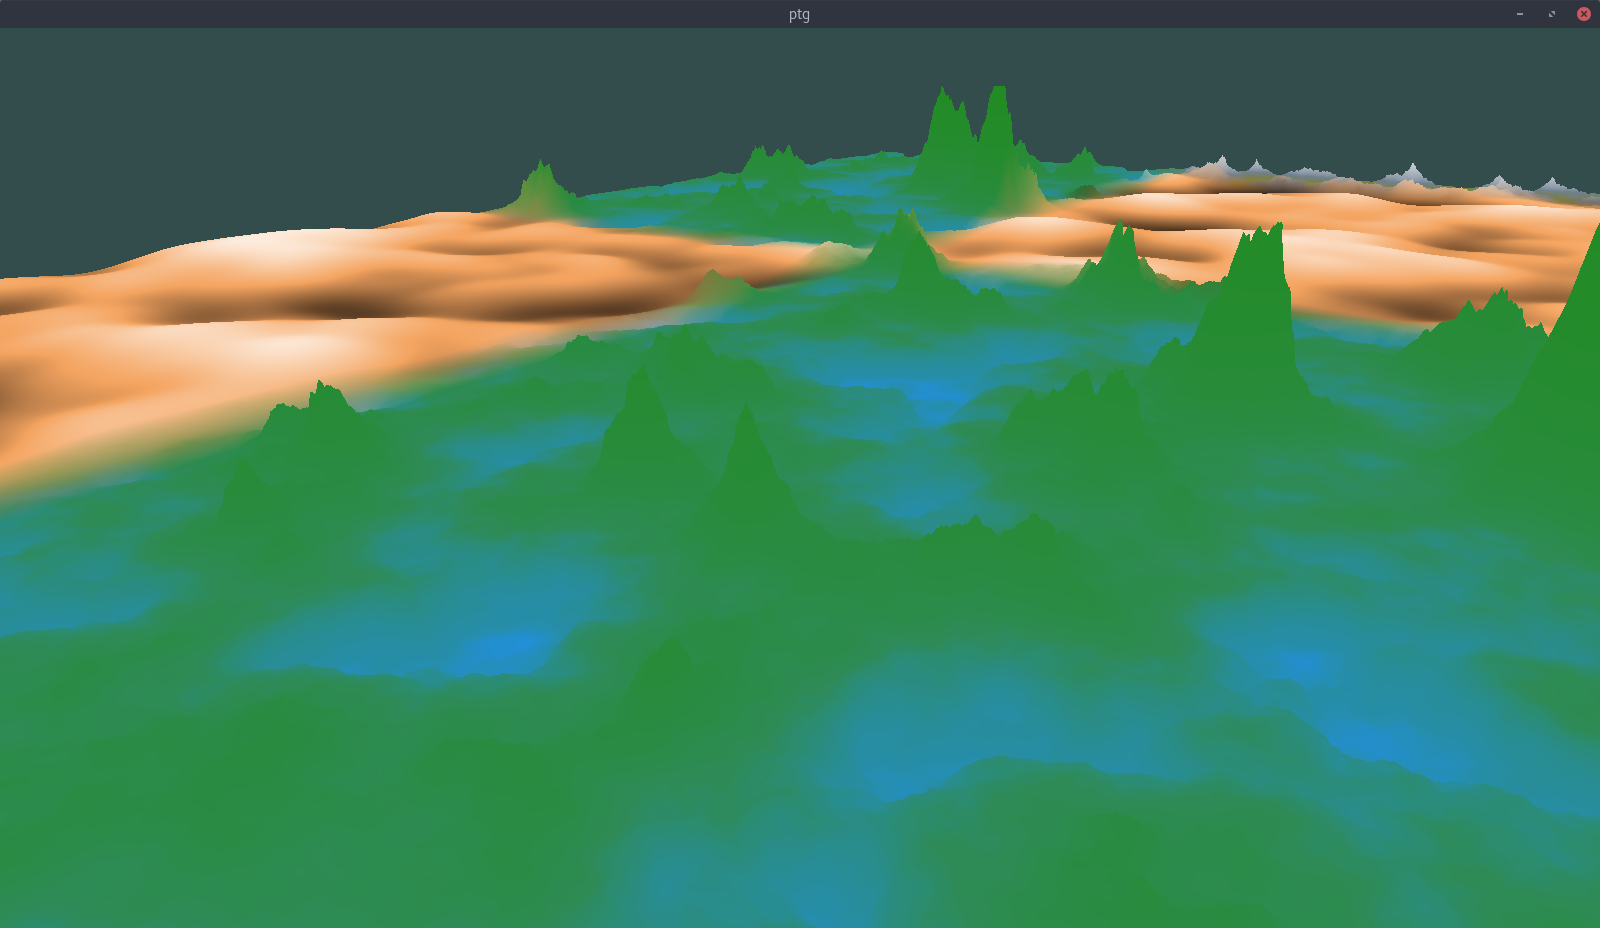
\includegraphics[width=0.48\textwidth]{figuras/resultados/b/resultSeed3Deltav05k2048b1500l128.png}\label{fig:b1500}}
     
     \caption{Tamanho de cada Bioma.}
     
     \label{fig:biomeComp}
     % usar \hspace{0.1cm}, é gambiarra mas funciona
\end{figure}

\begin{figure}[H]
     \centering
     \subfloat[][$l = 2$]{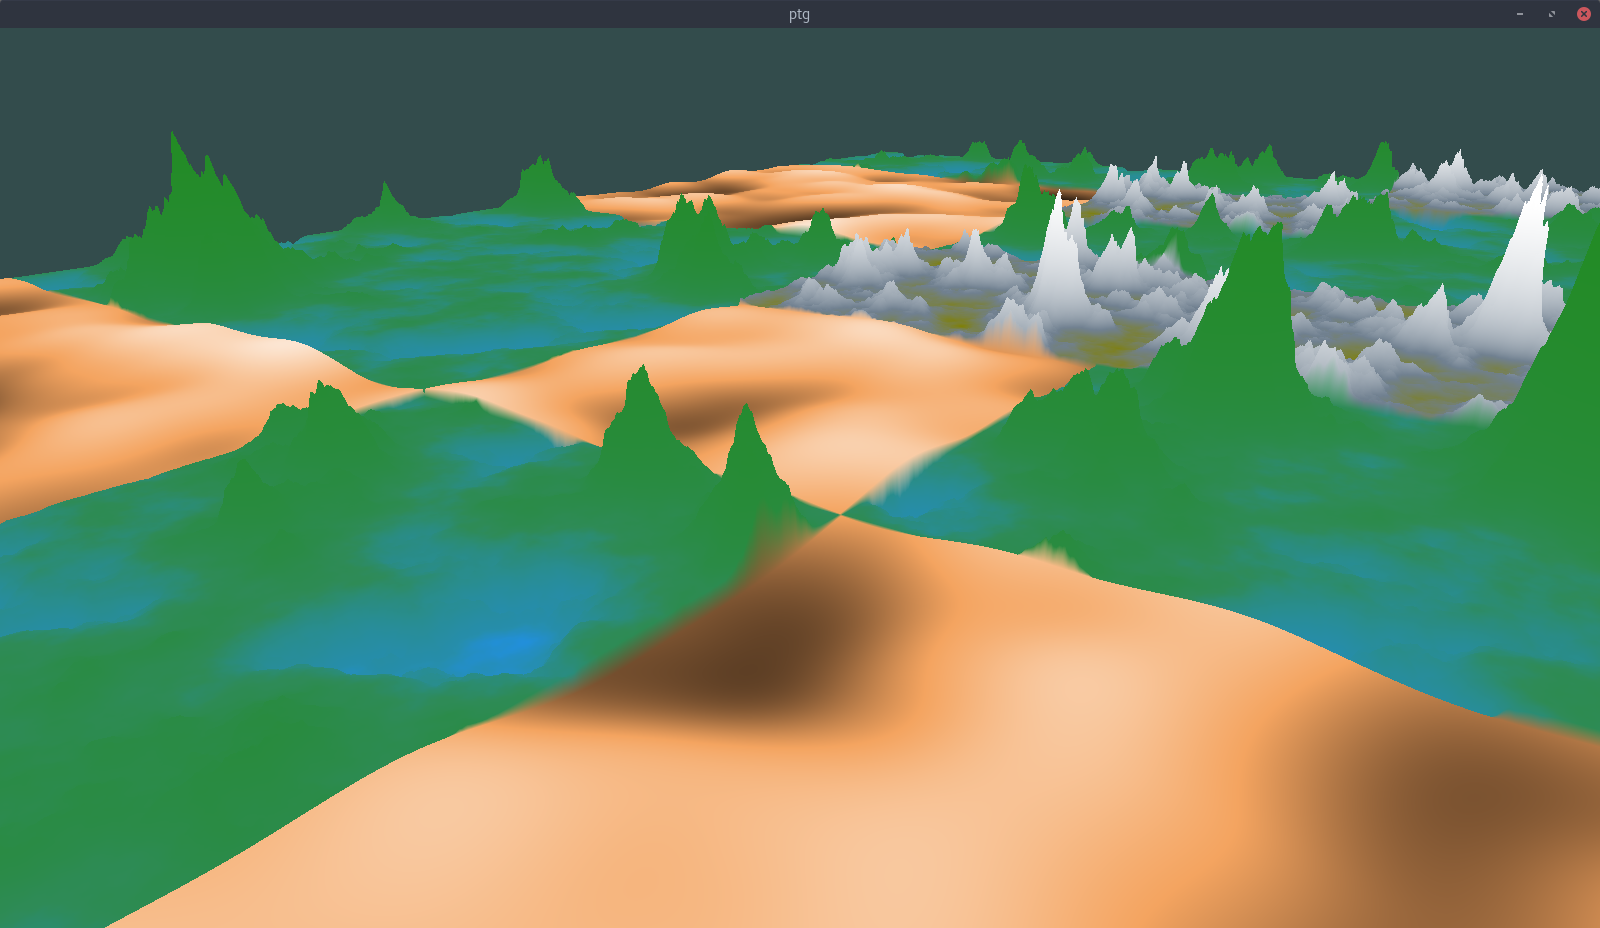
\includegraphics[width=0.48\textwidth]{figuras/resultados/l/resultSeed3Deltav05k2048b512l2.png}\label{fig:l2}}\hspace{0.1cm}
     \subfloat[][$l = 64$]{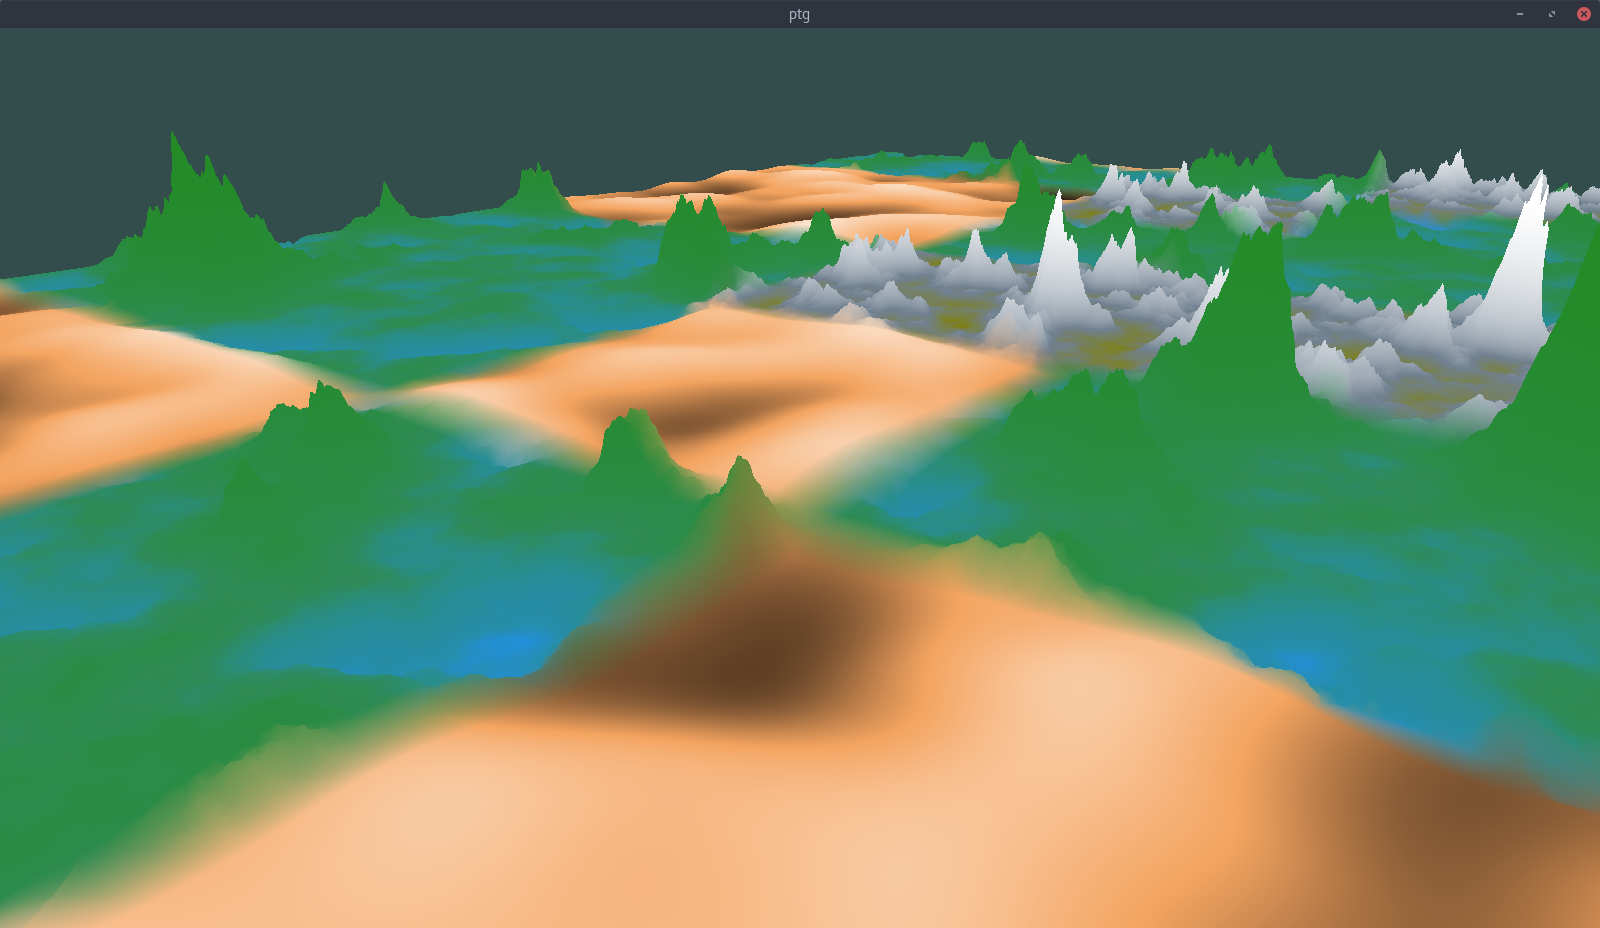
\includegraphics[width=0.48\textwidth]{figuras/resultados/l/resultSeed3Deltav05k2048b512l64.png}\label{fig:l64}}\\
     \subfloat[][$l = 128$]{\includegraphics[width=0.48\textwidth]{figuras/resultados/l/resultSeed3Deltav05k2048b512l128.png}\label{fig:l128}}\hspace{0.1cm}
     \subfloat[][$l = 256$]{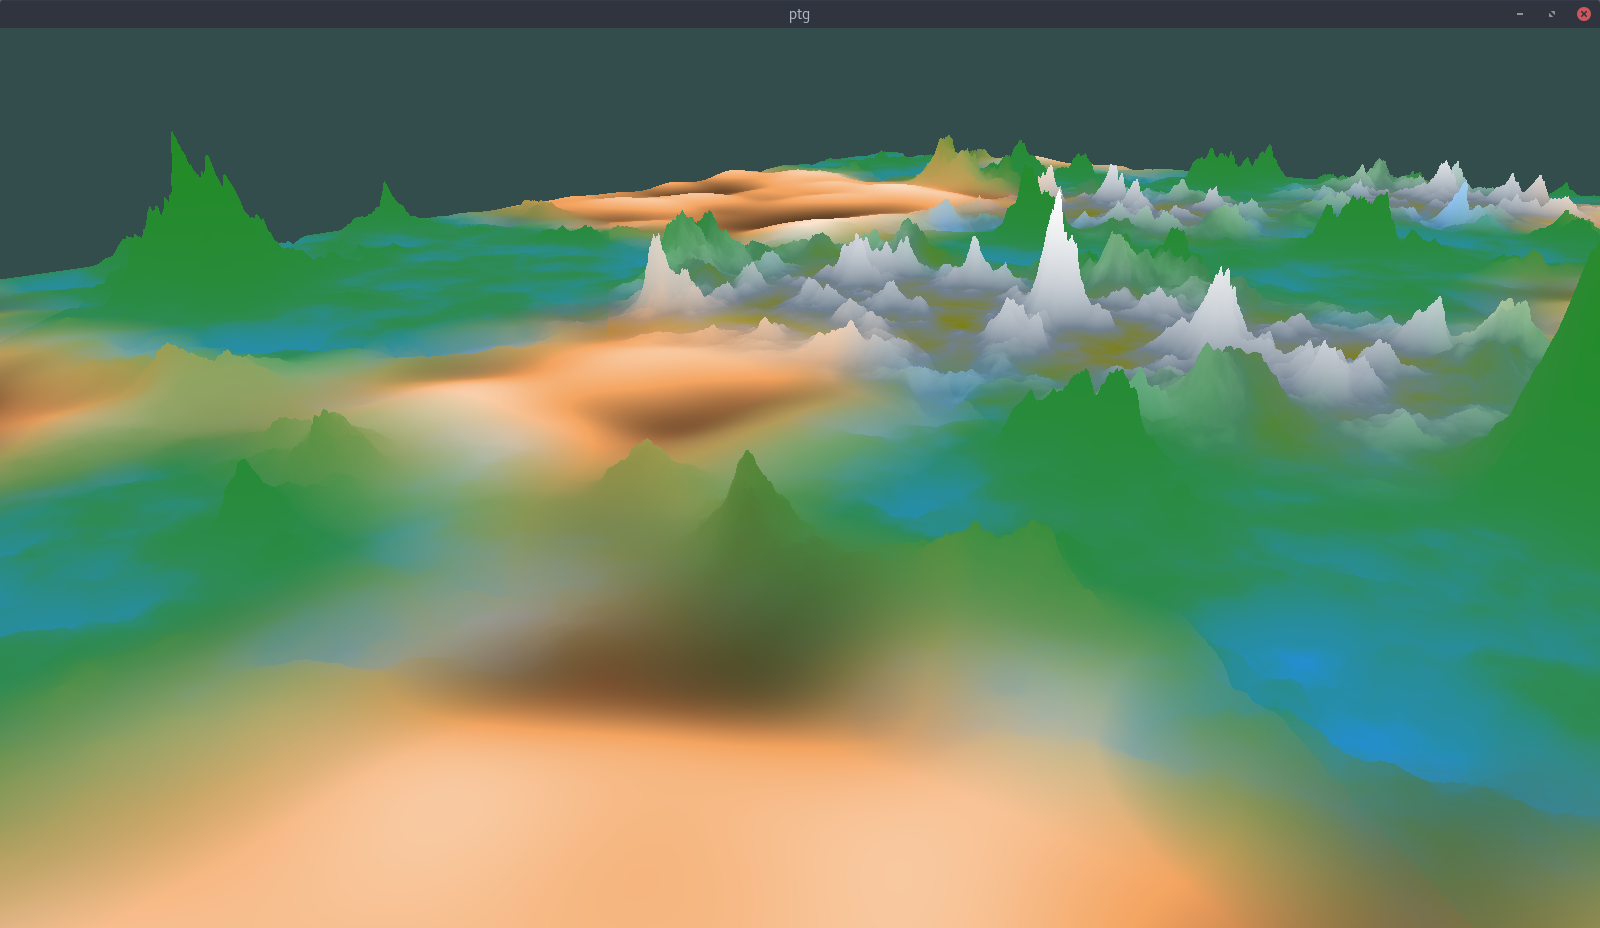
\includegraphics[width=0.48\textwidth]{figuras/resultados/l/resultSeed3Deltav05k2048b512l256.png}\label{fig:l256}}
     
     \caption{Alcance da fronteira.}
     
     \label{fig:lenghBioComp}
     % usar \hspace{0.1cm}, é gambiarra mas funciona
\end{figure}

\begin{figure}[H]
     \centering
     \subfloat[][$seed = 1$]{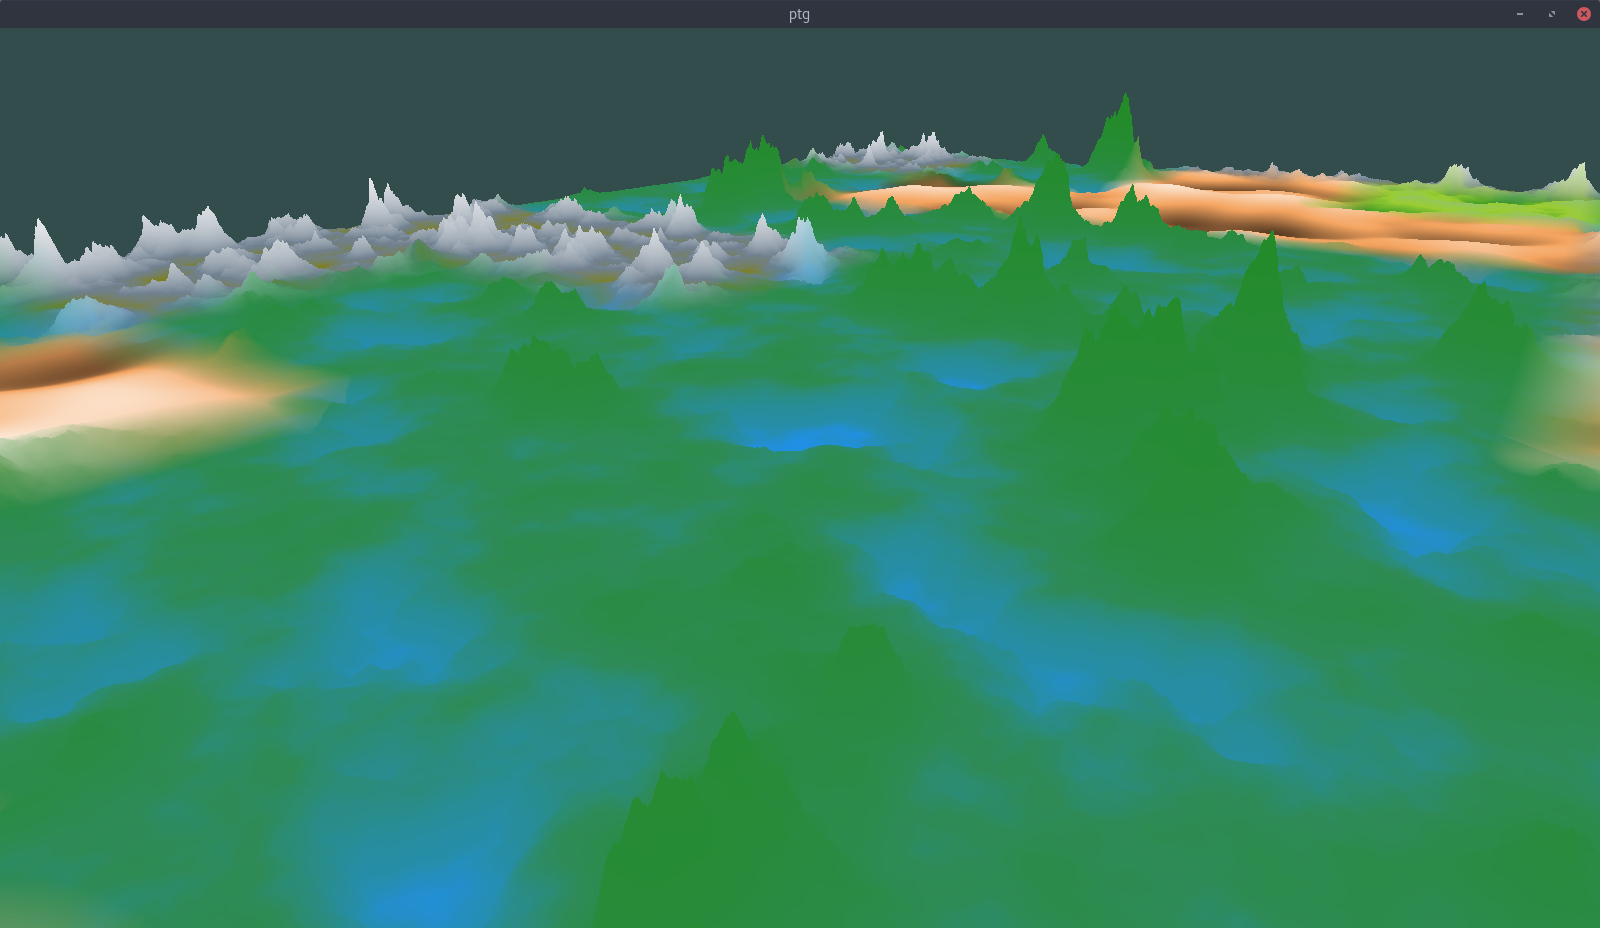
\includegraphics[width=0.48\textwidth]{figuras/resultados/seed/resultSeed1Deltav05k2048b512l128.png}\label{fig:seed1}}\hspace{0.1cm}
     \subfloat[][$seed = 2$]{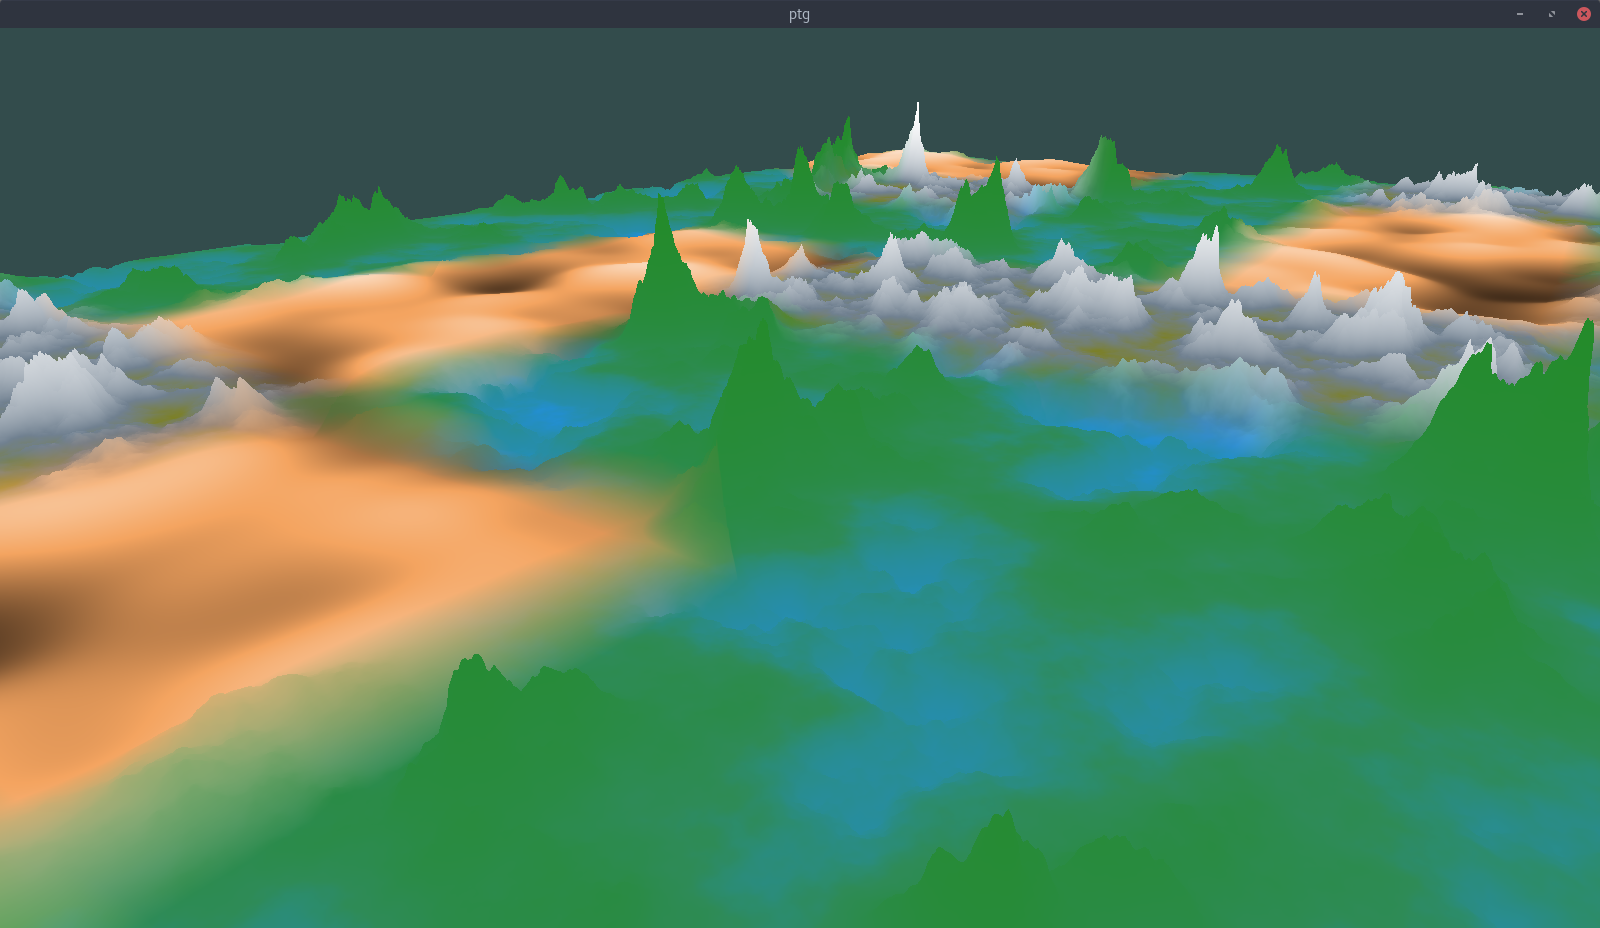
\includegraphics[width=0.48\textwidth]{figuras/resultados/seed/resultSeed2Deltav05k2048b512l128.png}\label{fig:seed2}}
     
     \caption{Semente para o motor de números pseudo aleatórios.}
     
     \label{fig:seedComp}
     % usar \hspace{0.1cm}, é gambiarra mas funciona
\end{figure}
%duvida 1: qual melhor pessoa para usar em frazes
%   nessa etapa precisamos (ingles)
%   nessa etapa é preciso
%   nessa etapa precisei
%   nessa etapa foi necessário       usar essa

%Conjunto de equações, recomendação do emílio
%\begin{align}
%    A \in Z^{2} \\
%    mix(A, B, c) &= (1-c) * A + c*B \\
%    mix(A, B, c) &= (1-c) * A + c*B \\
%\end{align}

\chapter{Implementação}

%Essa seção não é muito relevante para o resultado final, não sei se escrevo ela
\section{Configuração do Ambiente}

%Mover para fundamentação teórica
\subsection{Usando os Buffers do OpenGL e GLSL}

\subsubsection{Descrição dos vértices}
Um vértice $v$ é um conjunto de informações relacionadas a alguma unidade, %DEBUG: trocar o termo unidade
a informação necessária para este projeto é posição no espaço, então cada vértice
vai possuir uma posição notada por $v.pos$, e $v.pos$ é composto por 
$\{x, y, z\} \in \mathbb{Q}^3$. Um segundo dado será usado, a cor, vai ser uma 
informação auxiliar, usada para melhor vizialização dos resultados, 
representada por $\{r, g, b \in \mathbb{Q}:0 \leq r, g, b \leq 1\}$ onde cada um desses
vai referir a proporção de vermelho, verde e azul respectivamente.

\subsubsection{Implementação do sistema de Navegação}

\section{\textit{Terrain chunk}}
Representando um fragmento do terreno, o objeto \textit{Terrain chunk} é responsavel
por gerar uma malha para o terreno com $k^2$ vértices, o construtor pode receber 
a seguinte tupla para inicialização: 
$terrainChunk(seed, \Delta{v}, k, x_{s}, z_{s}, b, l)$
%referenciar as fatias do fernando
\begin{itemize}
    \item $seed \in \mathbb{N}$ representa a semente para começar o motor de números
    pseudo-aleatórios;
    \item $\Delta{v} \in \mathbb{Q}:0 < \Delta{v} < l/2$ é a distância entre vértices adjeacentes na
    projeção do plano $X \times Z$;
    \item $k \in \mathbb{N}>4$ é a quantidade de vértices em cada coluna ou 
    linha, a malha tem $k^2$ vértices;
    \item $x_{s} \in \mathbb{Q}:$ é o valor inicial no eixo $X$;
    \item $z_{s} \in \mathbb{Q}:$ é o valor inicial no eixo $Z$;
    \item $b \in \mathbb{N}>4:$ a área da região de cada bioma vai ser $b^2$;
    \item $l \in \mathbb{N}:1 < l < b/2$ distância para fronteira entre biomas ser interpolada.
\end{itemize}


Em cada execução da iplementação os valores que podem mudar de uma chunk para 
outra são apenas $x_{s}$ e $z_{s}$. Uma maneira de conseguir gerar terreno sobre demanda
é usando a localização da camera $(x_{c}, y_{c}, z_{c})$, quando ela se
aproxima de alguma borda da chunk atual
uma \textit{thread} é acionada pedidndo para calcular uma nova chunk, com os parâmetros
$terrainChunk(seed, \Delta{v}, k, x_{c}/\Delta{v} - k/2, z_{c}/\Delta{v} - k/2, b, l)$, assim que ela %debug: atualizar fórmula
estiver calculada a mesma começa a ser renderizada, substituindo a chunk anterior.
Antes de renderizar alguma chunk é necessário fazer uma translação com o vetor direção 
$(x_{s} * \Delta{v}, 0.0, z_{s} * \Delta{v})$, já que internamente cada chunk vai 
da posição $(0, 0)$ até $(\Delta{v}*(k-1), \Delta{v}*(k-1))$, mas representando a área 
no mundo $(x_{s}, z_{s})$ até $(x_{s} + \Delta{v}*(k-1), z_{s} + \Delta{v}*(k-1))$

\section{Criando Malha de Triângulos}
A maneira que um jogo renderiza seu terreno no final das contas é sobre uma
malha, uma malha é um conjunto de vértices que podem representar fragmentos
de uma superfície do terreno.

Para representar um segmento de plano precisamos de pelo menos $3$ vértices, 
já que com dois podemos apenas representar segmentos de retas. Um plano precisar
ter um mesmo vetor normal para todo o plano.

A malha segue pelo plano $X \times Z$, e cada vértice do plano vai ter uma altura
$y$ definida mais tarde por ruído. Se quisermos que o conjunto de pontos pertença
ao memos segmento de plano precisamos que os quatro pontos respeitem a mesma
equação do plano.%colocar referêrencia da malha de triângulos

Se usarmos como plano $4$ pontos em $\mathbb{Q}^3$
\begin{equation}\label{comp_sign_inter_sem_peso_aux}
    P = \{p_{0}(0, y_{0}, 0), p_{1}(0, y_{1}, 1), p_{2}(1, y_{2}, 0), p_{3}(1, y_{3}, 1)\}
\end{equation}
Para montar a equação do plano temos $\{y_{0}, y_{1}, y_{2}\}$ como valores livres e $y_{3}$
vai depender dos valores de $\{p_{0}, p_{1}, p_{2}\}, x_{3} e z_{3}$

%Aqui vai o cálculo da equação do plano ou do vetor normal para mostrar o que
%acabei de afirmar acima
%Calculando o vetor normal associado ao plano formado por $\{v0, v1, v2\}$
%$v0v1 = (0, y1-y0, 1)$
%$v0v2 = (1, y2-y0, 0)$

mas não é isso o objetivo, já que o ruído pode retornar valores para $y_{3}$
que não respeitem a equação do plano queremos que todos os pontos tenha valores de $y$
livres, portanto, será uma malha de triângulos. Então pro conjunto de vértices
acima temos dois triângulos associados:
$T_{1} = \{p_{0}, p_{1}, p_{2}\}, T_{2} = \{p_{3}, p_{1}, p_{2}\}$, que podem ser
vizualizados na figura \ref{fig:t1t2}. 
Desta maneira temos todos os pontos com $y$ livre.

\begin{figure}[H]
    \centering
    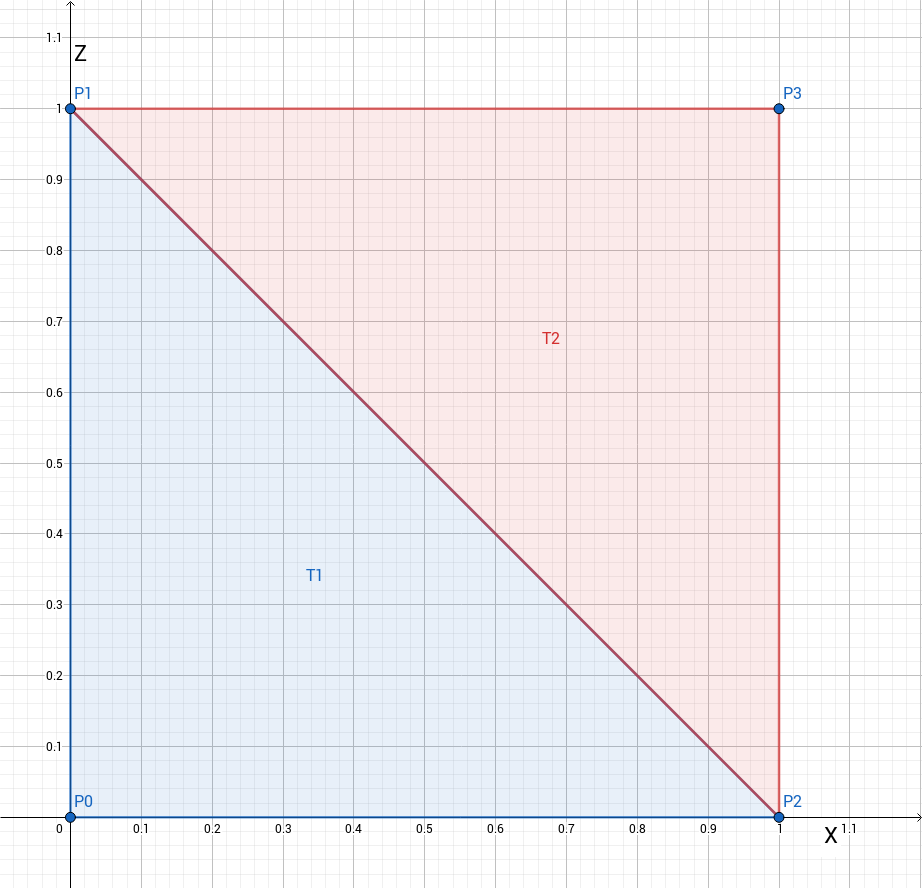
\includegraphics[width=0.5\textwidth]{figuras/t1t2.png}
    \caption{$T_{1}$ e $T_{2}$ projetados em $X \times Z$}
    \label{fig:t1t2}
\end{figure}


Então para montar um grid renderizavel usamos o algoritmo \ref{alg:genVectors}
$V$ é a estrutura que armazena os vértices, de $v_{0}$ até $v_{k^2-1}$ 
$E$ é a estrutura que armazena os índices, já que o \textit{OpenGL} precisa
saber a ordem de desenhar cada triângulo e quais vértices fazem parte dele, 
cada elemento de $e_{i} \in \mathbb{N}$ e a estrutura vai de $e_{0}$ até $e_{(k-1)^2 * 6 - 1}$.

A função \textit{hEvaluation}, vamos comentar mais adiante, ela retorna uma estrutura
com a altura e cor para algum ponto $(x, z)$.
 
\begin{algorithm}[H]\label{alg:genVectors}
    $|V| = k^2$\;
    \For{$i=0$ \KwTo $k-1$}{
        \For{$j=0$ \KwTo $k-1$}{
            $v_{i*k + j}.pos = (\Delta_{v} * i, hEvaluation(\Delta_{v} * i, \Delta_{v} * j).h, \Delta{v} * j)$\;
            $v_{i*k + j}.cor = hEvaluation(\Delta_{v} * i, \Delta_{v} * j).c$
        }
    }
    
    \For{$i=0$ \KwTo $k-2$}{
        \For{$j=0$ \KwTo $k-2$}{
            //posições em $V$ do primeio triângulo\;
            $E.$pushBack$(i*k +j)$\;
            $E.$pushBack$(i*k +j+1)$\;
            $E.$pushBack$((i+1)*k +j)$\;
            //posições em $V$ do segundo triângulo\;
            $E.$pushBack$((i+1)*k +j+1)$\;
            $E.$pushBack$(i*k +j+1)$\;
            $E.$pushBack$((i+1)*k +j)$\;
        }
    }
    \caption{Construção da coleção de vértices e índices.}
\end{algorithm}

\begin{figure}[H]
    \begin{figure}[H]
        \centering
        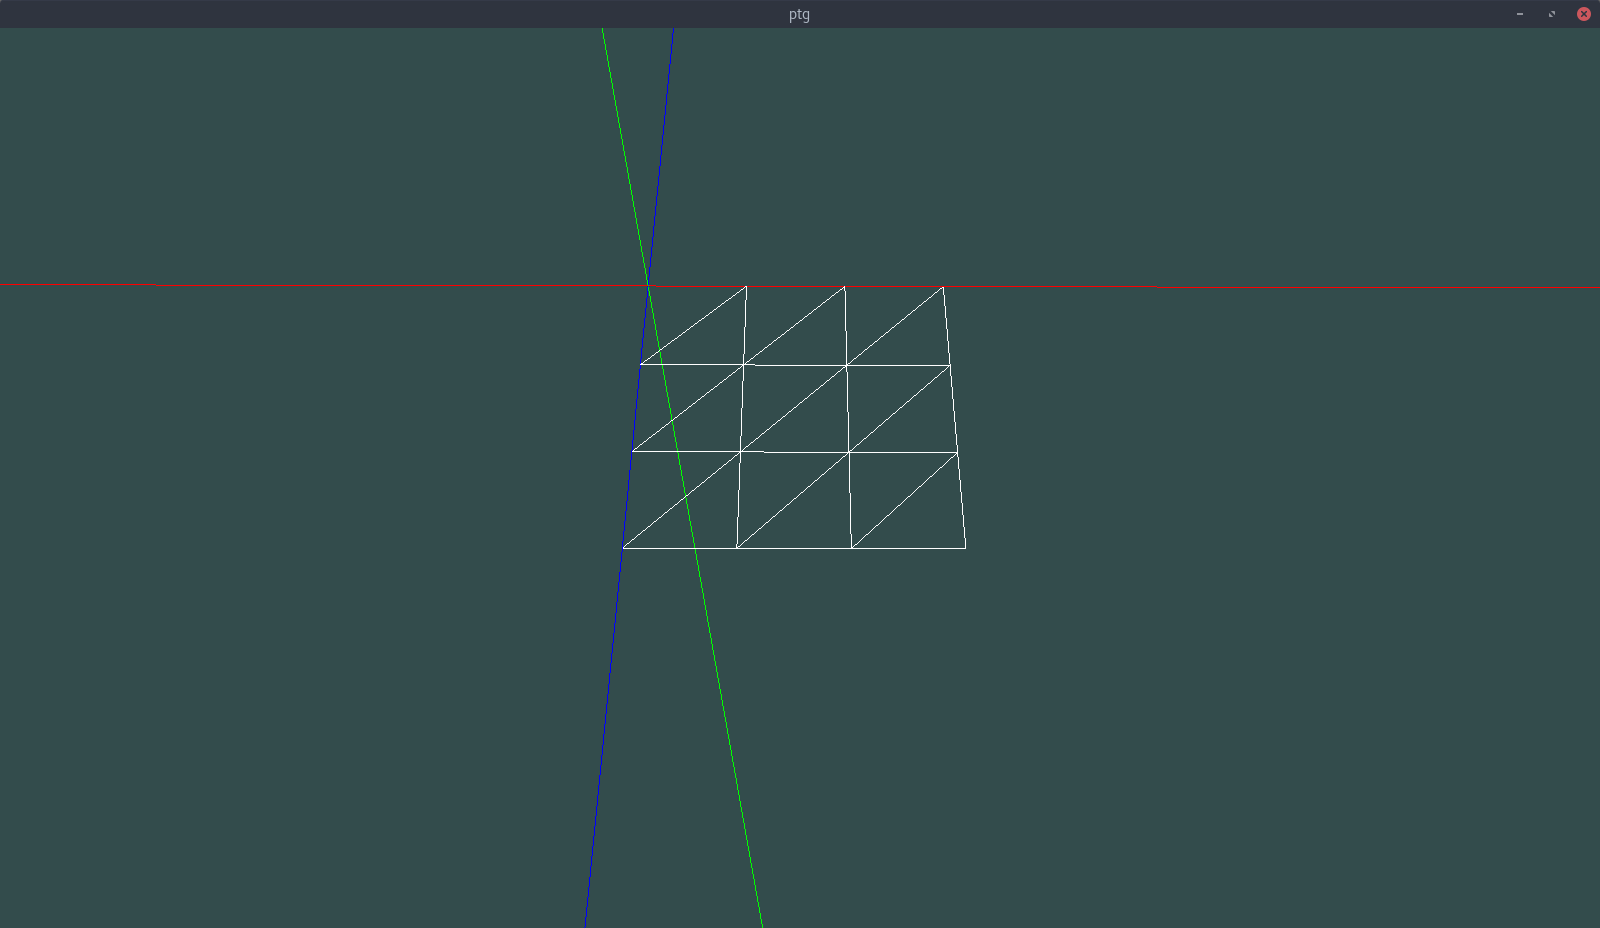
\includegraphics[width=0.2\textwidth]{figuras/k4d5.png}
        \caption{$T_{1}$ e $T_{2}$ projetados em $X \times Z$}
        \label{fig:k4d5}
    \end{figure}

    \begin{figure}[H]
        \centering
        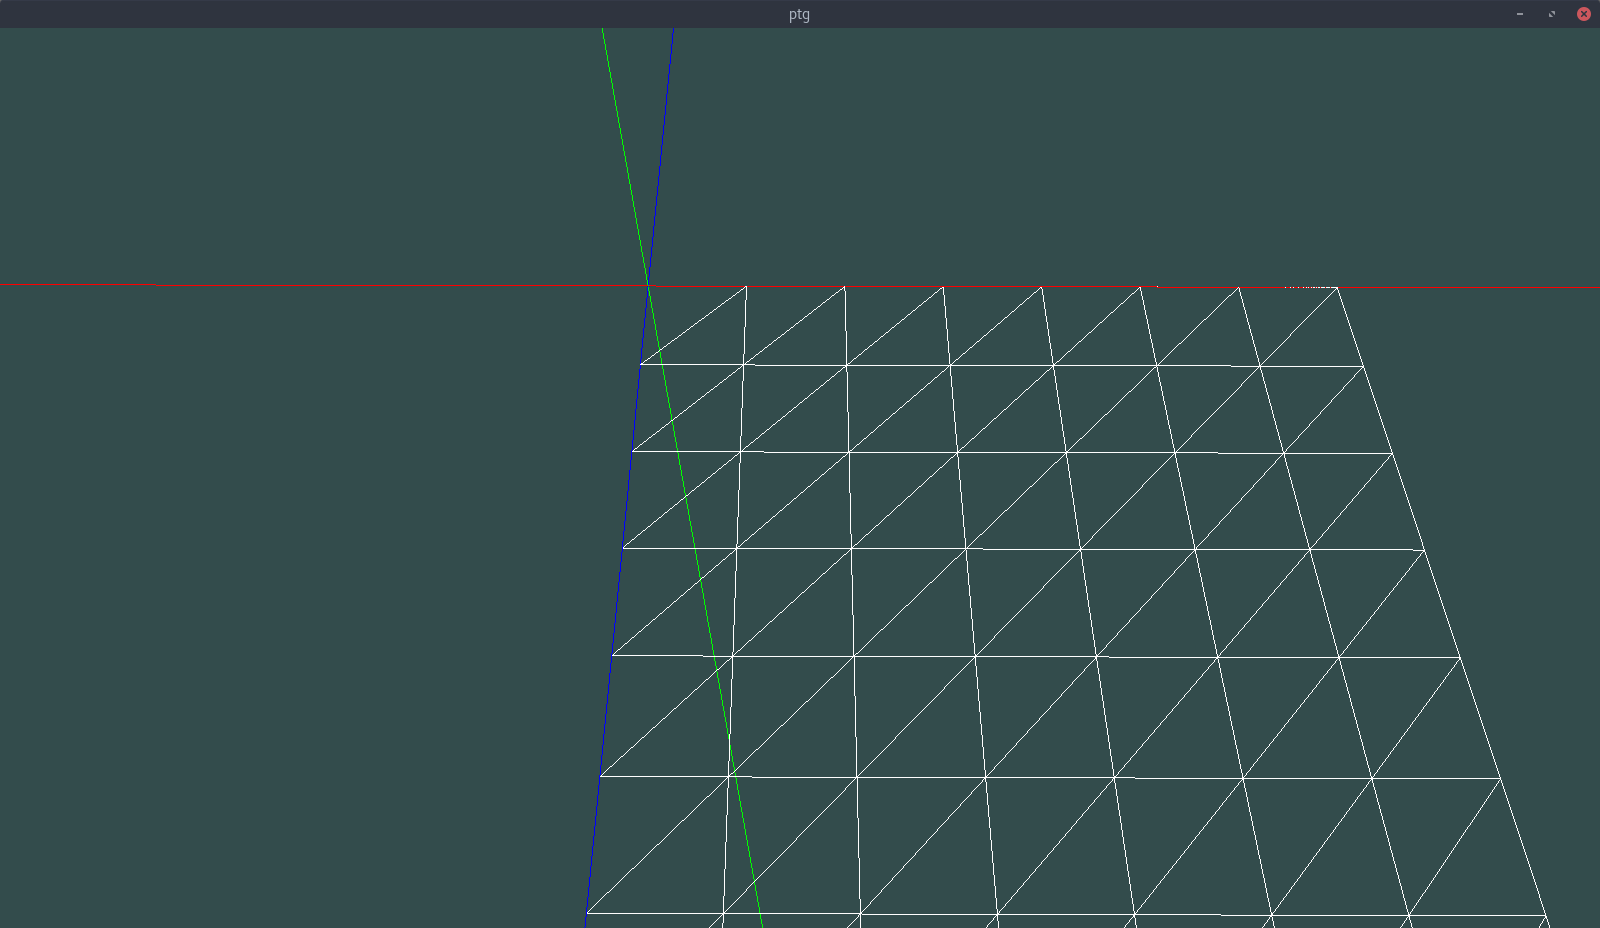
\includegraphics[width=0.2\textwidth]{figuras/k8d5.png}
        \caption{$T_{1}$ e $T_{2}$ projetados em $X \times Z$}
        \label{fig:k8d5}
    \end{figure}

    \begin{figure}[H]
        \centering
        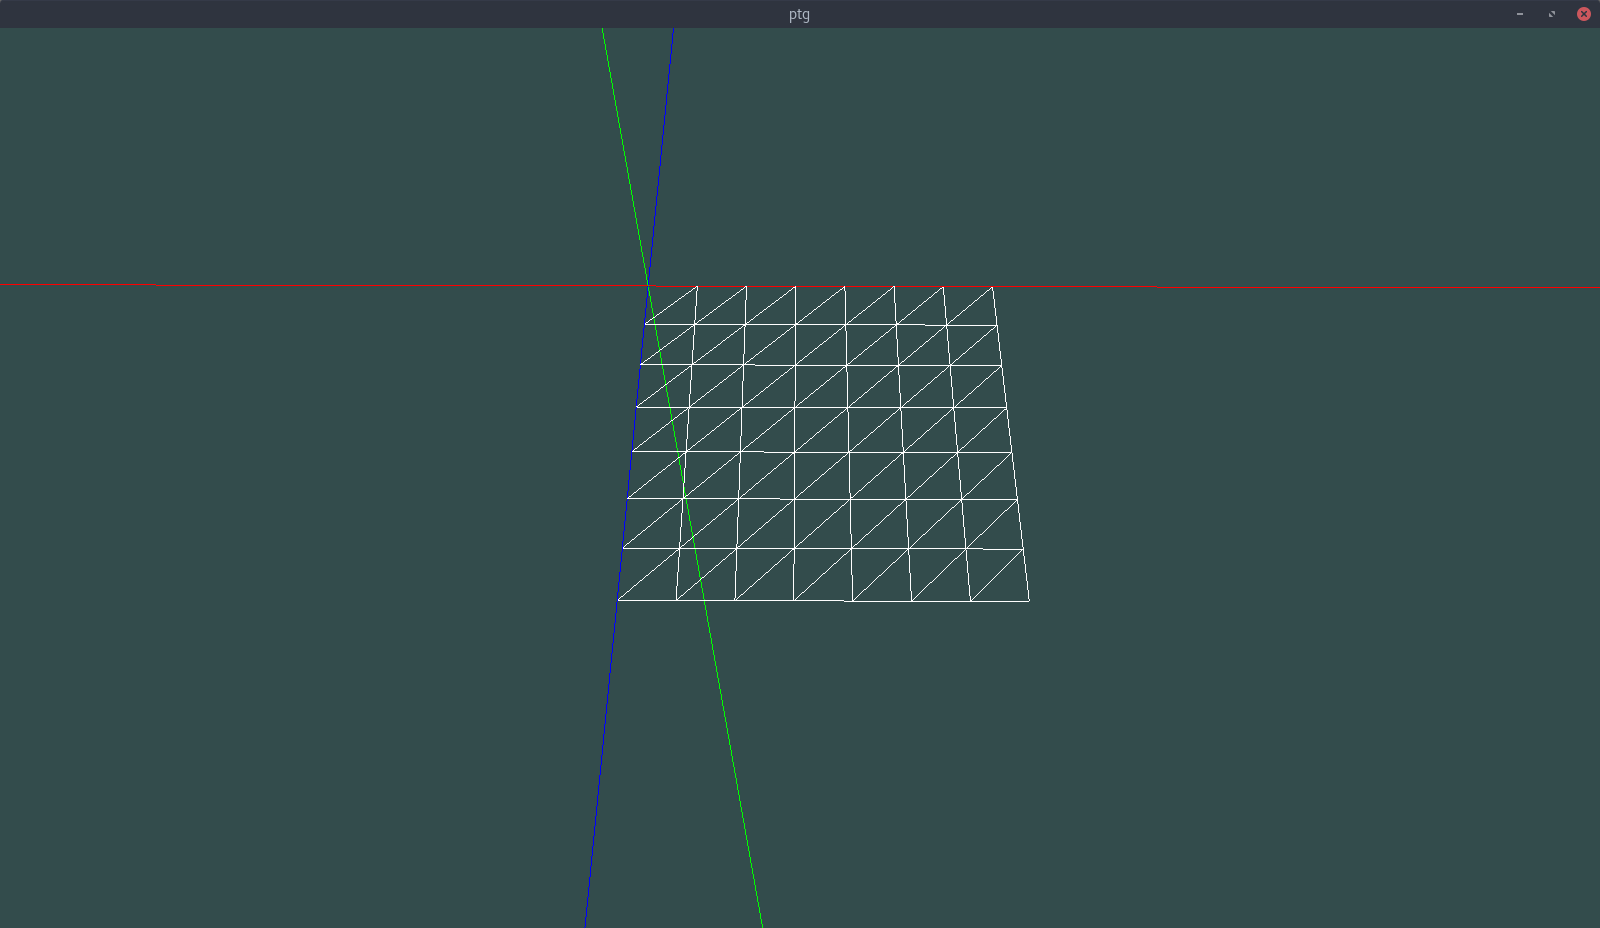
\includegraphics[width=0.2\textwidth]{figuras/k8d25.png}
        \caption{$T_{1}$ e $T_{2}$ projetados em $X \times Z$}
        \label{fig:k8d25}
    \end{figure}
    
\end{figure}




\section{Aplicando Ruído de Perlin nos Vértices}

\subsection{Manipulando ruído para criar Biomas}
\subsubsection{PLAINS}

\begin{figure}[H]
    \centering
    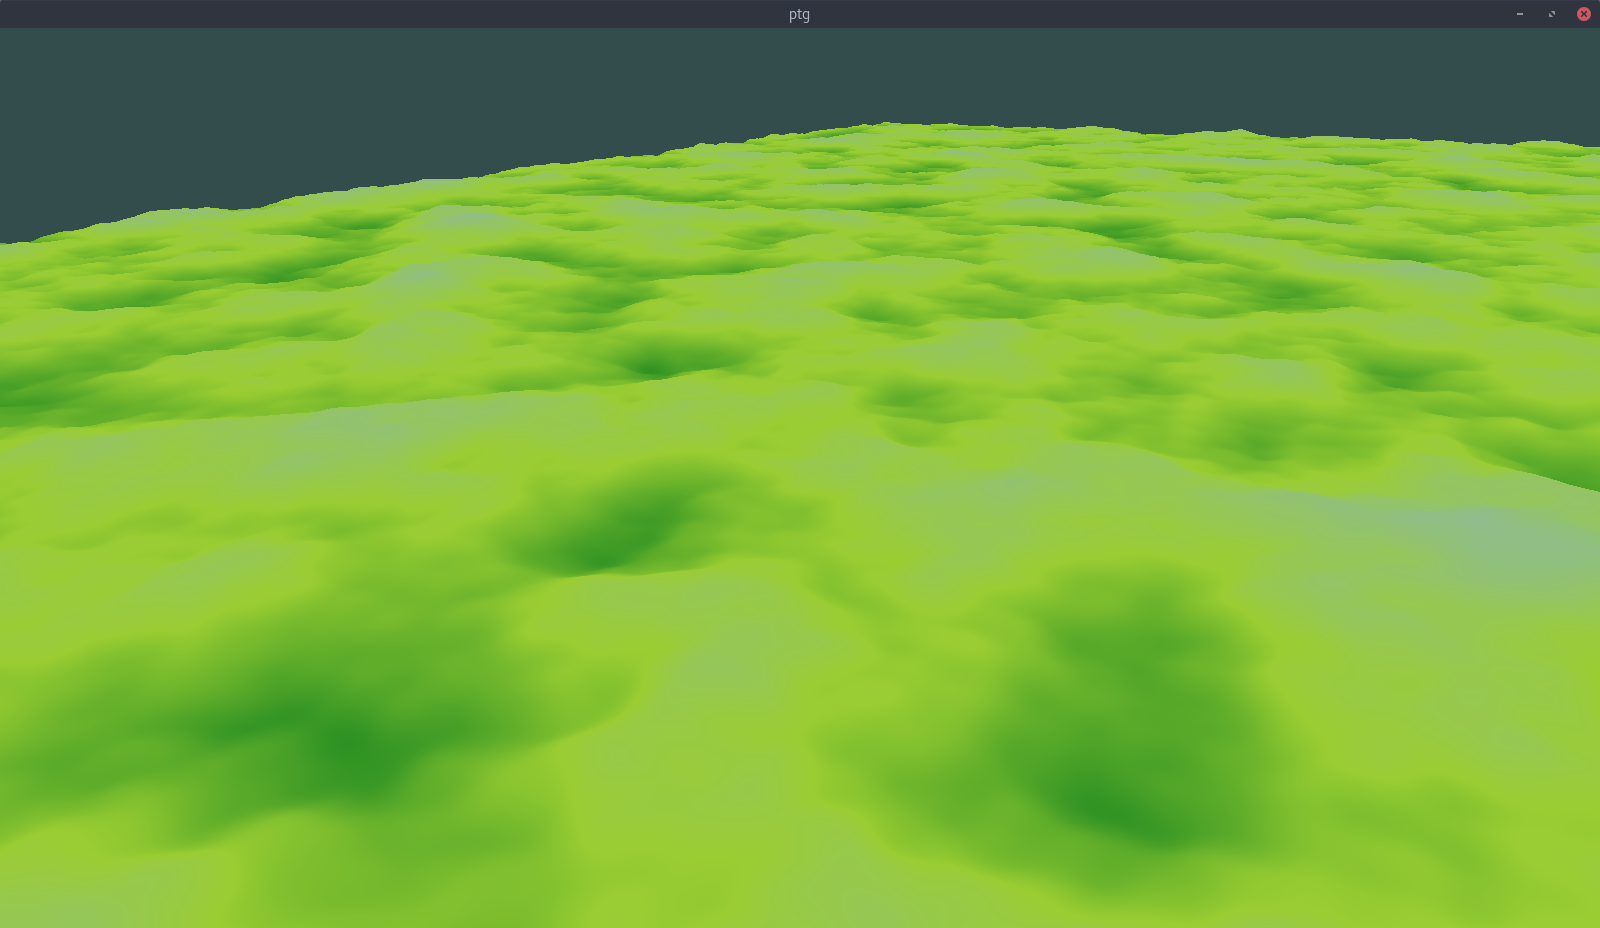
\includegraphics[width=0.5\textwidth]{figuras/bssPlains.png}
    \caption{Consumo}
    \label{fig:bssPlains}
\end{figure}

\subsubsection{MONTAINS}


\begin{figure}[H]
    \centering
    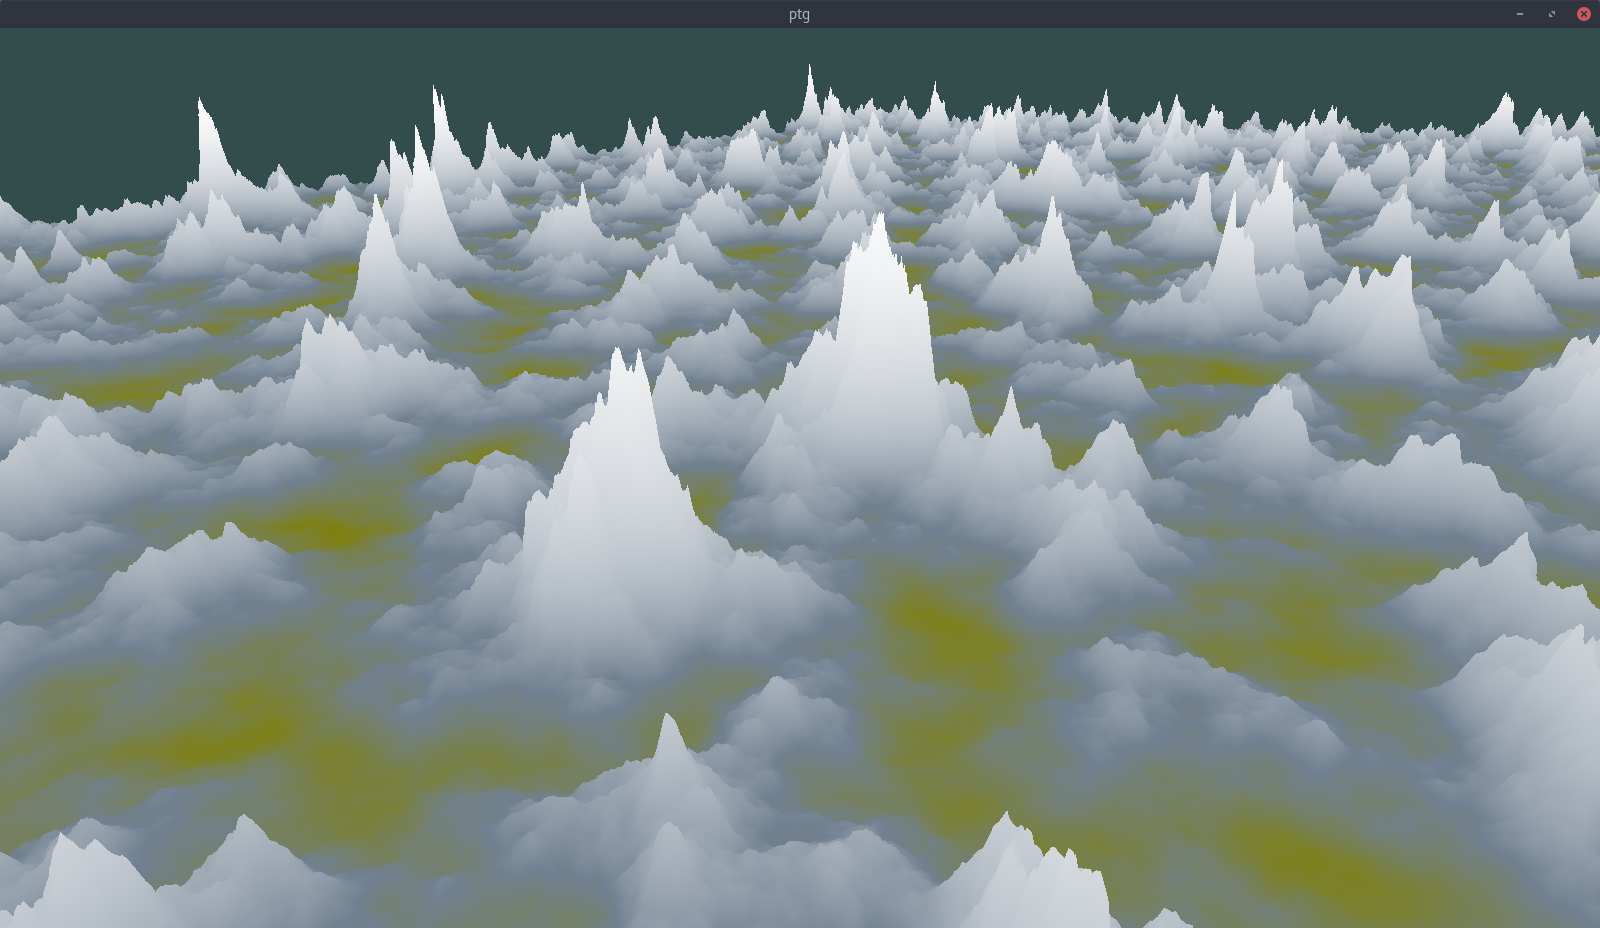
\includegraphics[width=0.5\textwidth]{figuras/bssMontains.png}
    \caption{Consumo}
    \label{fig:bssMontains}
\end{figure}

\subsubsection{VALLEY}


\begin{figure}[H]
    \centering
    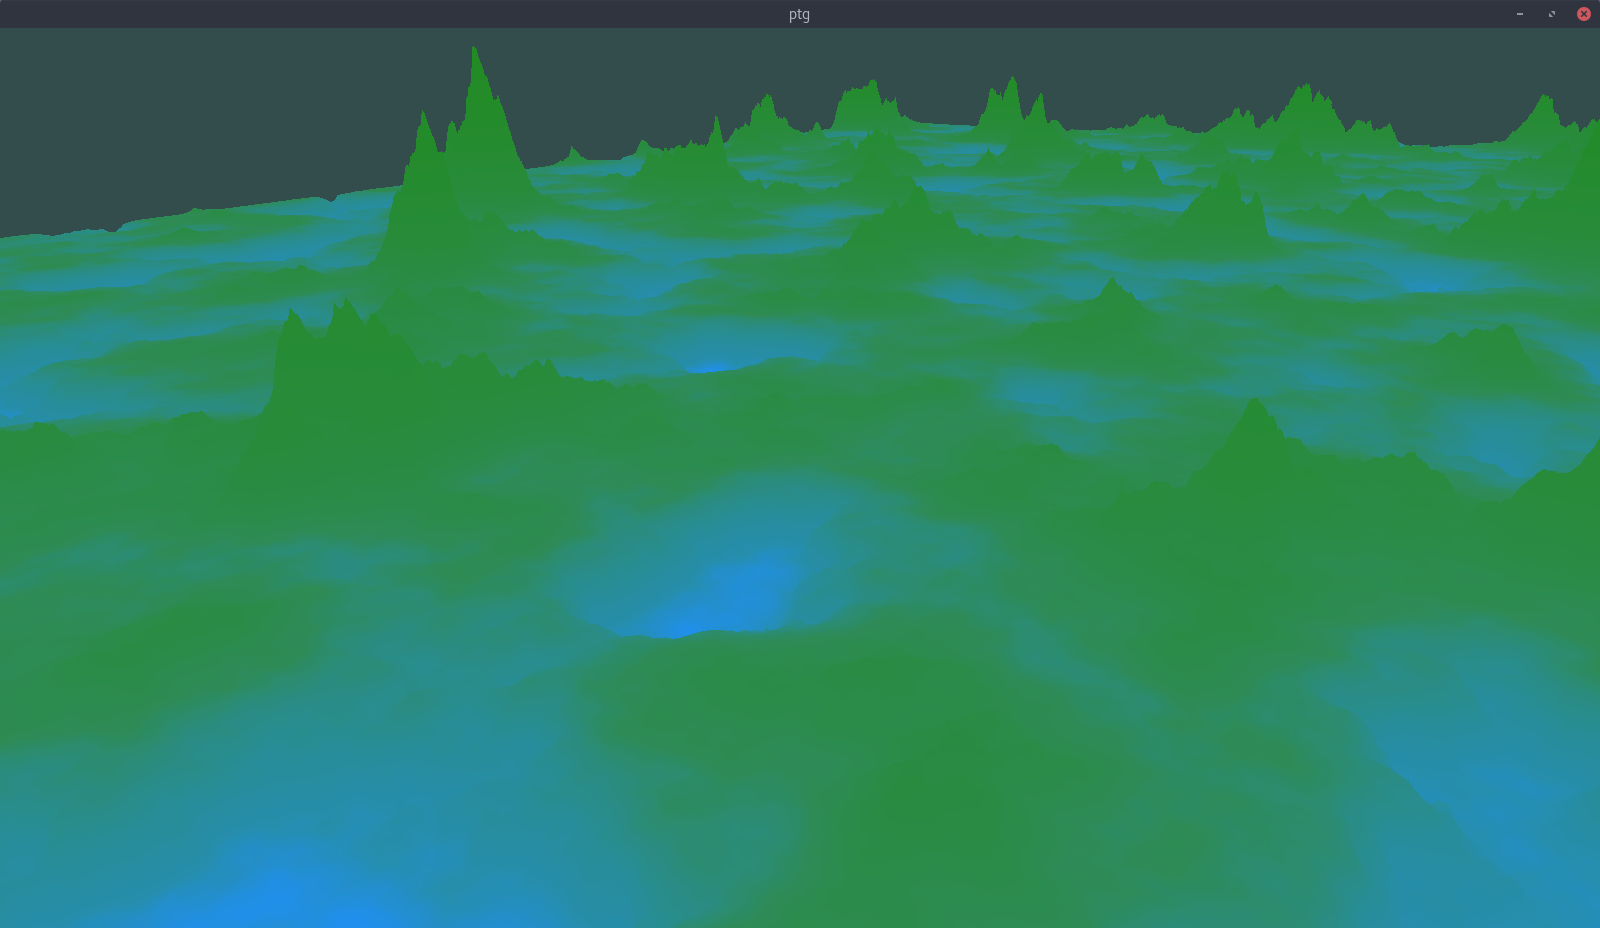
\includegraphics[width=0.5\textwidth]{figuras/bssValley.png}
    \caption{Consumo}
    \label{fig:bssValley}
\end{figure}

\subsubsection{DESERT}


\begin{figure}[H]
    \centering
    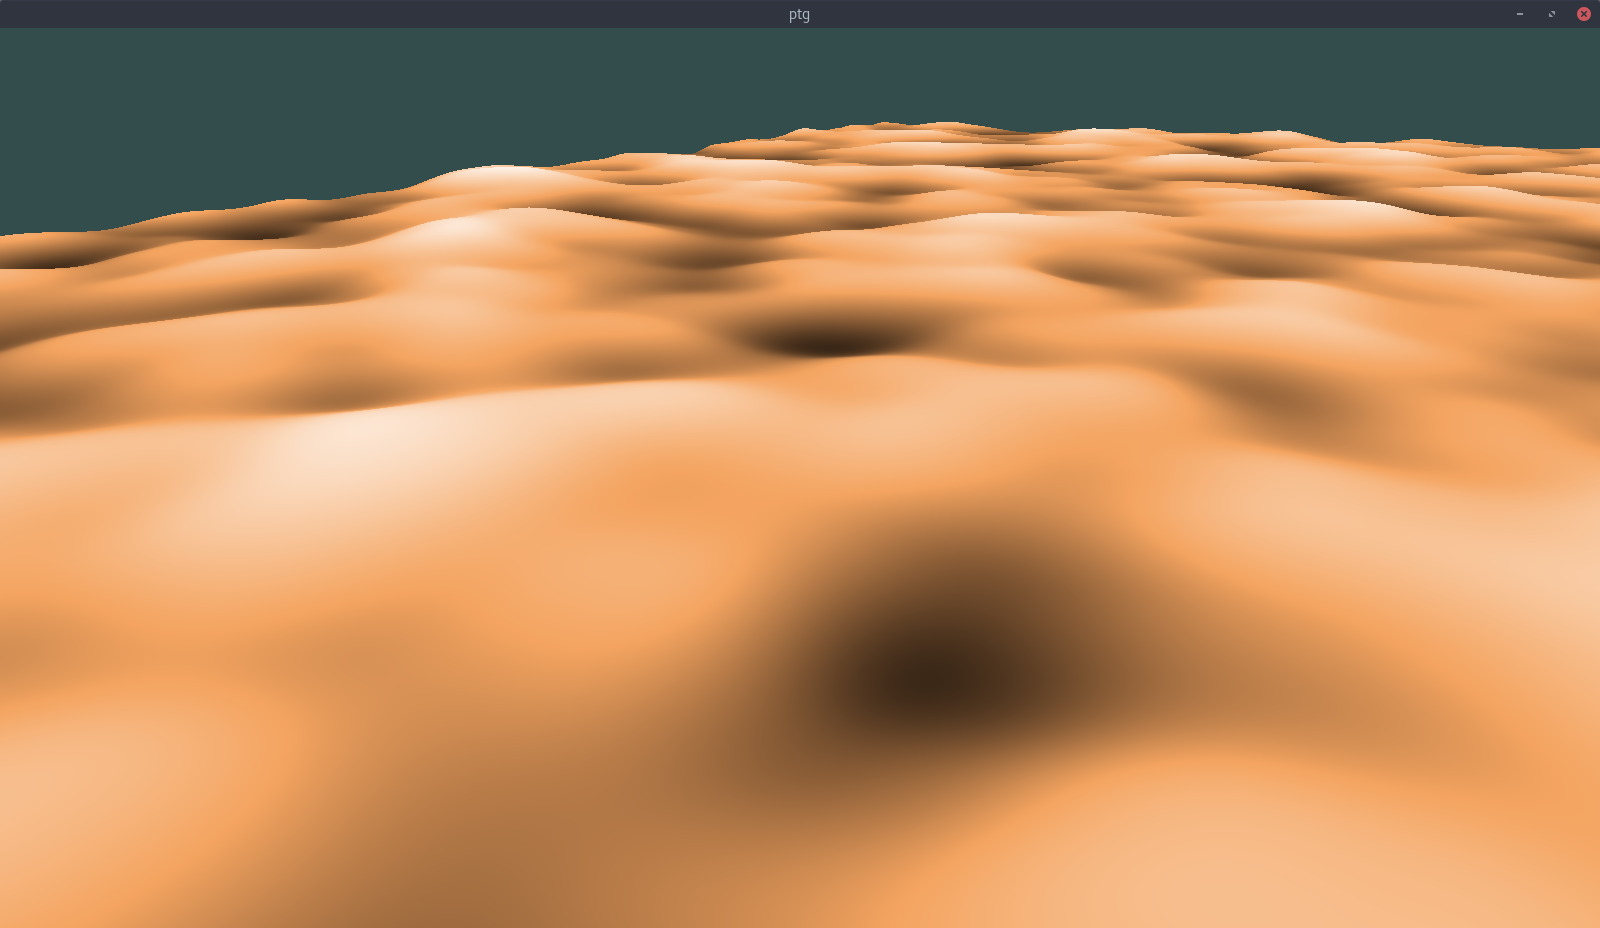
\includegraphics[width=0.5\textwidth]{figuras/bssDesert.png}
    \caption{Consumo}
    \label{fig:bssDesert}
\end{figure}

\subsubsection{CANYONS}


\begin{figure}[H]
    \centering
    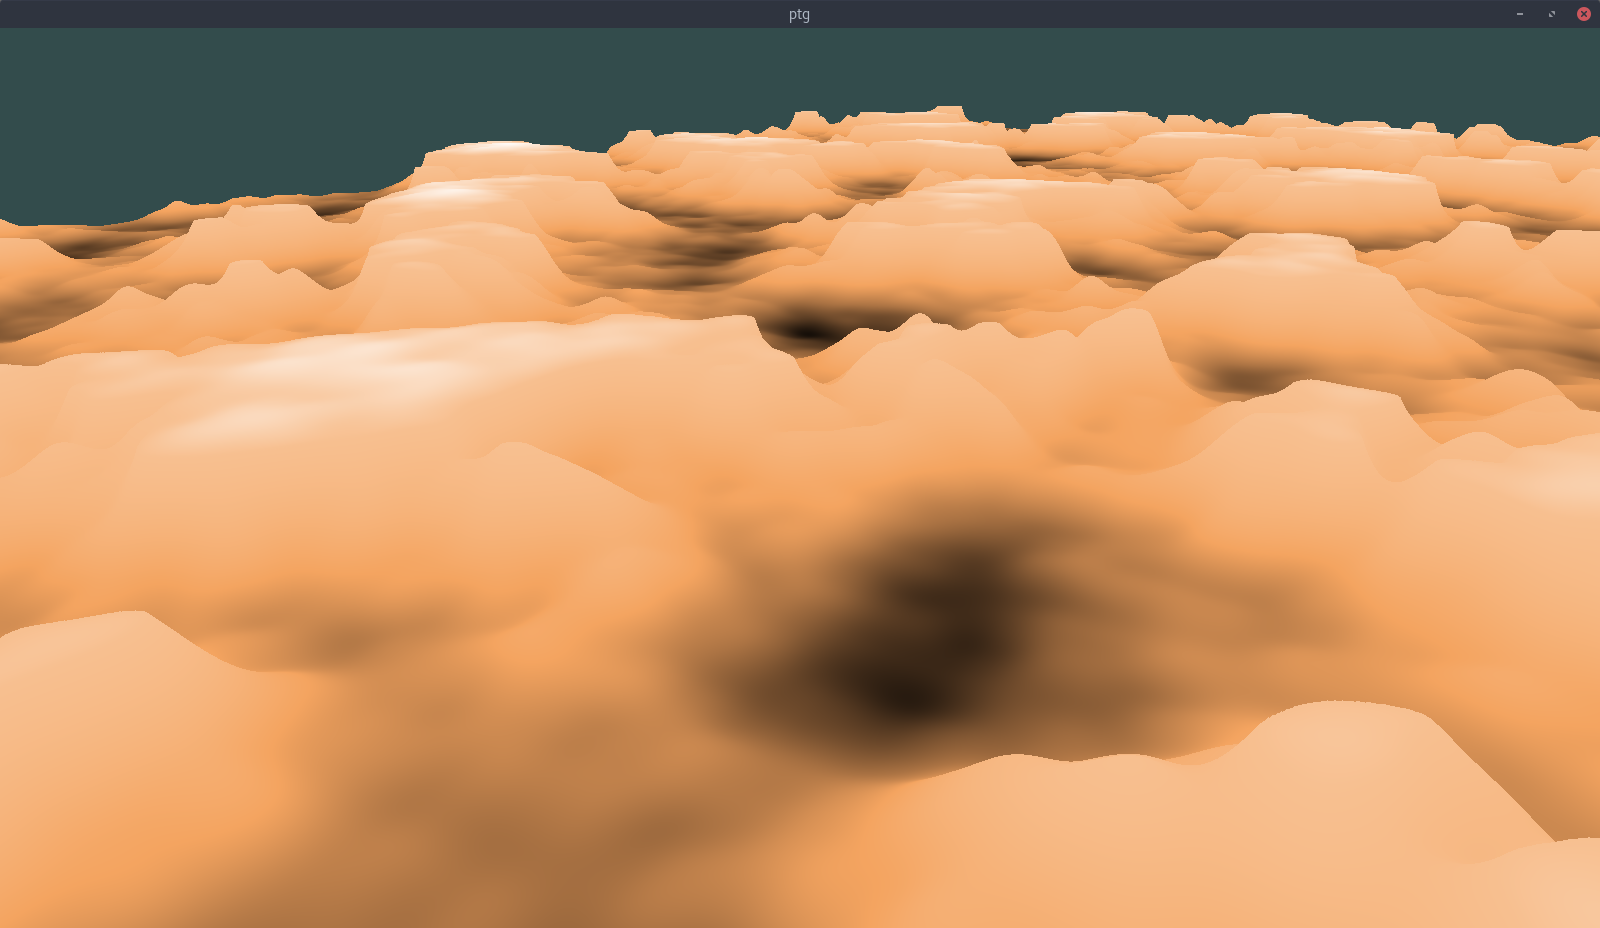
\includegraphics[width=0.5\textwidth]{figuras/bssCanyons.png}
    \caption{Consumo}
    \label{fig:bssCanyons}
\end{figure}

\section{Separando Áreas de Biomas}

\section{Detectando fronteira entre Biomas}
\begin{frame}{Conclusão}
    \begin{itemize} \setlength\itemsep{1em}
        \item Gerador de terreno para jogos:
        \begin{itemize} 
            \item Procedural, gerando terrenos vastos em pouco tempo
            \item Fronteiras contínuas e suavizadas, permite o personagem viajar entre biomas
        \end{itemize}
        \item Características configuráveis dos biomas:
        \begin{itemize}
            \item Raridade e fronteiras (intervalo)
            \item Proximidade ($fb$)
            \item Tamanho ($b$)
            \item Suavidade das fronteiras ($l$)
        \end{itemize}
        \item Novos biomas podem ser criados com diferentes $\theta, f$
        \begin{itemize}
            \item Adequado para outras características: vegetação, temperatura, etc
        \end{itemize}
    \end{itemize}
    
\end{frame}

\setlength{\baselineskip}{\baselineskip}

%%=============================================================================
%% Referências
%%=============================================================================
%\bibliographystyle{abbrv}------------------------------------------------------Original usava essa, mas sem informações da fonte, troca para abnt
%\bibliography{referencias/referencias}
\bibliographystyle{abnt}
\bibliography{referencias/referencias}



%IMPORTANTE: Se precisar usar alguma seção ou subseção dentro dos apêndices ou
%anexos, utilizar o comando \tocless para não adicionar no Sumário
%Exemplos: 
% \tocless\section{Histórico}
%%=============================================================================
%% Apêndices
%%=============================================================================
%\appendix
%\include{capitulos/apendicea}
%\include{capitulos/apendiceb}

%%=============================================================================
%% Anexos
%%=============================================================================
%\annex
%\include{capitulos/anexoa}

\end{document}
